% !TeX root = ./eLife_draft.tex

\documentclass[9pt]{nolife}
\usepackage[version=4]{mhchem}
\usepackage{siunitx}
\title{Fundamental limits on the rate of bacterial growth and their influence on proteomic composition}
\author[$\dagger$, 1]{Nathan M. Belliveau}
\author[$\dagger$, 2]{Griffin Chure}
\author[3]{Christina L. Hueschen}
\author[4]{Hernan G. Garcia}
\author[5]{Jane Kondev}
\author[6]{Daniel S. Fisher}
\author[1, *]{Julie A. Theriot}
\author[7, 8, *]{Rob Phillips}
\affil[1]{Department of Biology, Howard Hughes Medical Institute, University of Washington, Seattle, WA}
\affil[2]{Department of Applied Physics, California Institute of Technology, Pasadena, CA, USA}
\affil[3]{Department of Chemical Engineering, Stanford University, Stanford, CA, USA}
\affil[4]{Department of Molecular Cell Biology and Department of Physics, University of California Berkeley, Berkeley, CA, USA}
\affil[5]{Department of Physics, Brandeis University, Waltham, MA, USA}
\affil[6]{Department of Applied Physics, Stanford University, Stanford, CA, USA}
\affil[7]{Division of Biology and Biological Engineering, California Institute of Technology, Pasadena, CA, USA}
\affil[8]{Department of Physics, California Institute of Technology, Pasadena, CA, USA}
\affil[*]{Co-corresponding authors. Address correspondence to phillips@pboc.caltech.edu and jtheriot@uw.edu}
\affil[$\dagger$]{These authors contributed equally to this work}

\begin{document}
\maketitle
\begin{abstract}
Recent years have seen a deluge of experiments dissecting the relationship
between bacterial growth rate, cell size, and protein content, quantifying
the abundance of proteins across growth conditions with unprecedented
resolution. However, we still lack a rigorous understanding of what sets the
scale of these quantities and when protein abundances should (or should not)
depend on growth rate. Here, we seek to quantitatively understand this
relationship across a collection of \textit{Escherichia coli} proteomic data
sets covering $\approx$ 4000 proteins and 36 growth rates. We estimate
the basic requirements for steady-state growth by considering key processes
in nutrient transport, energy generation, cell envelope biogenesis, and the
central dogma. From these estimates, ribosome biogenesis emerges as a primary
determinant of growth rate. We expand on this assessment by exploring a model of proteomic
regulation as a function of the nutrient supply, revealing a mechanism that
ties cell size and growth rate to ribosomal content.

\end{abstract}

% !TeX root = ./eLife_draft.tex

\section{Introduction}
The observed range of bacterial growth rates is enormously diverse. In natural
environments, some microbial organisms may double only once per year
\citep{mikucki2009} while in comfortable laboratory conditions, growth can be
rapid with several divisions per hour \citep{schaechter1958}. This six
order-of-magnitude difference in time scales of growth encompasses different
microbial species and lifestyles, yet even for a single species such as
\textit{Escherichia coli}, the growth rate can be modulated over a
large scale by tuning the type and amount of nutrients in the growth medium
\citep{liu2005a}. This remarkable plasticity in growth rate illustrates the
intimate relationship between environmental conditions and the rates at which
cells convert nutrients into new cellular material -- a relationship that has
remained a major topic of inquiry in bacterial physiology for over a century
\citep{jun2018}.

A key discovery in bacterial physiology of the past 70 years was the
identification of bacterial "growth laws" \citep{schaechter1958}; empirical
relationships that relate the bacterial growth rate to the protein and RNA
composition of the intracellular milieu in a number of different species.
Over the past decade, a flurry of work \citep{molenaar2009, scott2010,
klumpp2014, basan2015, dai2016, erickson2017} has examined these growth laws
at a quantitative level, developing a series of phenomenological models from
which the growth laws naturally emerge. In parallel, a "molecular revolution"
in biology has yielded an increasingly refined molecular census of the cell,
particularly for bacteria such as the microbial workhorse \textit{E. coli}
\citep{schmidt2016, davidi2016a}. In light of the now expansive trove of
quantitative biological data, we can revisit several of the evergreen
questions about bacterial growth and physiology that were originally raised
by microbiologists in the middle of the 20th century. Specifically, what
biological processes are the primary determinants for how quickly bacterial
cells can grow and reproduce? Why do cells modulate the absolute numbers and
relative ratios of their molecular constituents as a function of changes in
growth rate or nutrient availability?

In this work, we begin by considering these two questions from two distinct
angles. First, as a result of an array of high-quality proteome-wide
measurements of \textit{E. coli} under diverse growth conditions, we have
generated a census that allows us to explore how the number of key molecular
players change as a function of growth rate. Here, we have assembled a singular
data set of protein copy numbers using measurements collected over the past
decade via mass spectrometry \citep{schmidt2016, peebo2015, valgepea2013} or
ribosomal profiling \citep{li2014} of the composition of the \textit{E. coli}
proteome across a gamut of growth rates. Due to notable changes in cell size and
cellular composition as a function of growth rate \citep{bremer2008,
taheriaraghi2015}, as well as differences in normalization and standardization
schemes used in each experimental work, substantial care was taken to ensure
consistency on a per cellular basis (see the Appendix for a detailed analysis
and additional discussion). To our knowledge, this compiled and curated dataset
represents the most comprehensive view to date of the \textit{E. coli} proteome,
covering $\approx$ 4000 proteins and 36 unique growth rates, with the observed
abundance of any given protein being directly comparable between data sets and
across growth rates. This allows us to interrogate  the \textit{E. coli}
specific physiology underlying the observed abundances while  minimizing the
effects of experimental noise, as  $\approx$ 75\% of the  proteins are observed
in at least two separate datasets.

Second, by compiling molecular turnover rate measurements for many of the
fundamental processes associated with bacterial growth, we make quantitative
estimates of a handful of key cellular processes (schematized in
\FIG{categories}) to determine whether our current understanding of the
kinetics of these processes are sufficient to explain the magnitude of the
observed protein copy numbers across conditions (see \BOX{estimate_rules}
describing the philosophy behind this approach). The census, combined with
these estimates, provide a window into the question of whether the rates of
central processes such as energy generation or DNA synthesis vary
systematically as a function of cell growth rate by altering protein copy
number.

Throughout our estimates, we consider an archetypal growth rate of $\approx$
0.5 hr$^{-1}$ corresponding to a doubling time of $\approx$ 5000 seconds, as
the data sets examined here heavily sample this growth regime. While we
formulate point estimates for the protein abundances at this division time,
we also consider how these values will vary at other growth rates due to
changes in cell size, surface area, and chromosome copy number
\citep{taheriaraghi2015, harris2018}. For the majority of the processes
considered, we find that the protein copy numbers appear tuned for the task
of cell doubling across a continuum of growth rates. Thus, our understanding
of the kinetics of various biological processes is sufficient to
quantitatively explain the observed abundances of these proteins.

% From these estimates, it emerges that translation, particularly the synthesis of
% ribosomal proteins, is a plausible candidate that limits the rate of cellular
% growth in \textit{E. coli}.

From these estimates, it emerges that translation,  particularly the synthesis of ribosomal proteins is a
plausible candidate that limits the rate of cellular growth in \textit{E. coli}.
We reach this conclusion by considering that ribosome synthesis is 1) a rate
limiting step for the \textit{fastest} bacterial division, and  2) the main
determinant of bacterial growth rate across  nutrient conditions associated with
moderate to fast growth rates. In addition, a strict dependence between the
maximal growth rate and ribosomal mass fraction coincides with the regime where
the growth laws appear most valid \citep{amir2017, scott2010}. This enables us
to suggest that the long-observed correlation between growth rate and cell size
\citep{schaechter1958, si2017} can be simply attributed to the increased
absolute number of ribosomes per cell under conditions supporting extremely
rapid growth. To better understand how the observed alterations in absolute
protein abundances, and in particular, changes in ribosome copy number,
influence growth rate across different nutrient conditions we consider a minimal
model of cellular growth. Our conclusions from these analyses provide important
insight into how \textit{E. coli} regulates growth across conditions of
differing nutrient availability and identifies fundamental constraints in
bacterial growth more broadly.






\begin{figure}
    \centering{
    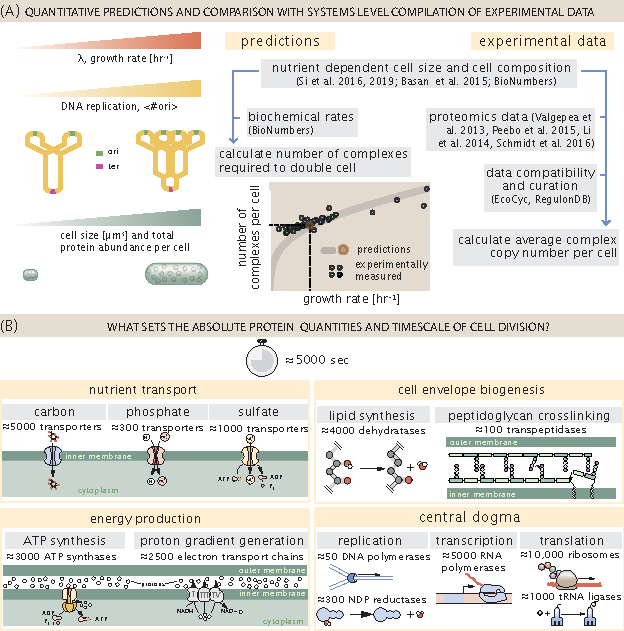
\includegraphics{main_figs/fig1_schematic_categories_grouped.pdf}
    \caption{\textbf{Transport and synthesis processes necessary for cell division.}
            We consider an array of processes necessary for a cell to double its
            molecular components, broadly grouped into four classes. These
            categories are (A) nutrient transport across the cell membrane, (B) cell envelope
            biogenesis, (C) energy production (namely, ATP synthesis), and (D) processes associated with the central dogma.
            Numbers shown are the approximate number of complexes of each type
            observed at a growth rate of 0.5 hr$^{-1}$, or a cell doubling time
            of $\approx$ 5000 s.}
    \label{fig:categories}
    }
\end{figure}

\section{Uptake of Nutrients}
In order to build new cellular mass, the molecular and elemental building blocks
must be scavenged from the environment in different forms. Carbon, for example,
is acquired via the transport of carbohydrates and sugar alcohols with some
carbon sources receiving preferential treatment in their consumption
\citep{monod1947}. Phosphorus, sulfur, and nitrogen, on the other hand, are
harvested primarily in the forms of inorganic salts, namely phosphate, sulfate,
and ammonia \citep{jun2018, assentoft2016, stasi2019, antonenko1997,
rosenberg1977, willsky1973}. All of these compounds have different
permeabilities across the cell membrane \cite{phillips2018} and  most require some energetic
investment either via ATP hydrolysis or through the proton electrochemical
gradient to bring the material across the hydrophobic cell membrane. Given the
diversity of biological transport mechanisms and the vast number of inputs
needed to build a cell, we begin by considering transport of some of the most
important cellular ingredients: carbon, nitrogen, oxygen, hydrogen, phosphorus,
and sulfur.

The elemental composition of \textit{E. coli} has received much quantitative
attention over the past half century \citep{neidhardt1991, taymaz-nikerel2010,
heldal1985, bauer1976}, providing us with a starting point for estimating the
copy numbers of various transporters. While there is some variability in the
exact elemental percentages (with different uncertainties), we can estimate that
the dry mass of a typical \textit{E. coli} cell is $\approx$ 45\% carbon (BNID:
100649, \cite{milo2010}), $\approx$ 15\% nitrogen (BNID: 106666,
\cite{milo2010}), $\approx$ 3\% phosphorus (BNID: 100653, \cite{milo2010}), and
1\% sulfur (BNID: 100655, \cite{milo2010}). In the coming paragraphs, we will
engage in a dialogue between back-of-the-envelope estimates for the numbers of
transporters needed to facilitate these chemical stoichiometries and the
experimental proteomic measurements of the biological reality. Such an approach
provides the opportunity to test if our biological knowledge is sufficient to
understand the scale at which these complexes are produced. Specifically, we
will make these estimates considering a modest doubling time of 5000 s, a growth
rate of $\approx$ 0.5 hr$^{-1}$, the range in which the majority of the
experimental measurements reside.

\subsection{Nitrogen Transport}
Before we begin our back-of-the-envelope estimations, we must address which
elemental sources must require proteinaceous transport, meaning that the cell
cannot acquire appreciable amounts simply via diffusion across the membrane.
The permeability of the lipid membrane to a large number of solutes has been
extensively characterized over the past century. Large, polar
molecular species (such as various sugar molecules, sulfate, and phosphate) have
low permeabilities  while small, non-polar compounds (such as oxygen, carbon
dioxide, and ammonia) can readily diffuse across the
membrane. Ammonia, a primary source of nitrogen in typical laboratory
conditions, has a permeability on par with water ($\approx 10^5$ nm/s,
BNID:110824 \cite{milo2010}). In particularly nitrogen-poor
conditions, \textit{E. coli} expresses a transporter (AmtB) which appears to aid in
nitrogen assimilation, though the mechanism and kinetic details of transport
are still a matter of debate \citep{heeswijk2013a, khademi2004}. Beyond ammonia,
another plentiful source of nitrogen come in the form of glutamate, which has it's
own complex metabolism and scavenging pathways. However, nitrogen is plentiful
in the growth conditions examined in this work, permitting us to neglect
nitrogen transport as a potential rate limiting process in cell division in
typical experimental conditions. We direct the reader to the supplemental
information for a more in-depth discussion of permeabilities and a series of
calculations revealing that active nitrogen transport can be neglected for the
purposes of this article.

\subsection{Carbon Transport}
We begin our estimations with the most abundant element in \textit{E. coli}
by mass, carbon. Using $\approx$ 0.3 pg as the typical \textit{E. coli} dry
mass (BNID: 103904, \cite{milo2010}), we estimate that $\approx 10^{10}$
carbon atoms must be brought into the cell in order to double all of the
carbon-containing molecules (\FIG{carbon_tport}(A, top)). Typical laboratory
growth conditions, such as those explored in the aforementioned proteomic
data sets, provide carbon as a single class of sugar such as glucose,
galactose, or xylose to name a few. \textit{E. coli} has evolved myriad
mechanisms by which these sugars can be transported across the cell membrane.
One such mechanism of transport is via the PTS system which is a highly
modular system capable of transporting a diverse range of sugars
\citep{escalante2012}. The glucose-specific component of this system
transports $\approx$ 200 glucose molecules per second per transporter (BNID:
114686, \cite{milo2010}). Making the assumption that this is a typical sugar
transport rate, coupled with the need to transport 10$^{10}$ carbon atoms, we
arrive at the conclusion that on the order of 1,000 transporters must be
expressed in order to bring in enough carbon atoms to divide in 5000 s,
diagrammed in the top panel of \FIG{carbon_tport}(A). This estimate, along
with the observed average number of the PTS system carbohydrate transporters present in the
proteomic data sets \citep{schmidt2016, peebo2015,valgepea2013,li2014}, is
shown in \FIG{carbon_tport}(A). While we estimate 1500 transporters are
needed with a 5000 s division time, we can abstract this calculation to consider
any particular growth rate given knowledge of the cell density and volume as a
function of growth rate and direct the reader to the SI for more information. As
revealed in \FIG{carbon_tport}(A), experimental measurements exceed the estimate
by several fold, illustrating that transport of carbon into the cell is not
rate limiting for cell division. Abstracting this point estimate at 5000 s to a
continuum of growth rates (grey line in \FIG{carbon_tport}(A)) reveals an excess
of transporters at other growth rates, though in rapid growth regimes, the
abundance is below our simple estimate.
\begin{figure}
    \begin{fullwidth}
    \centering{
    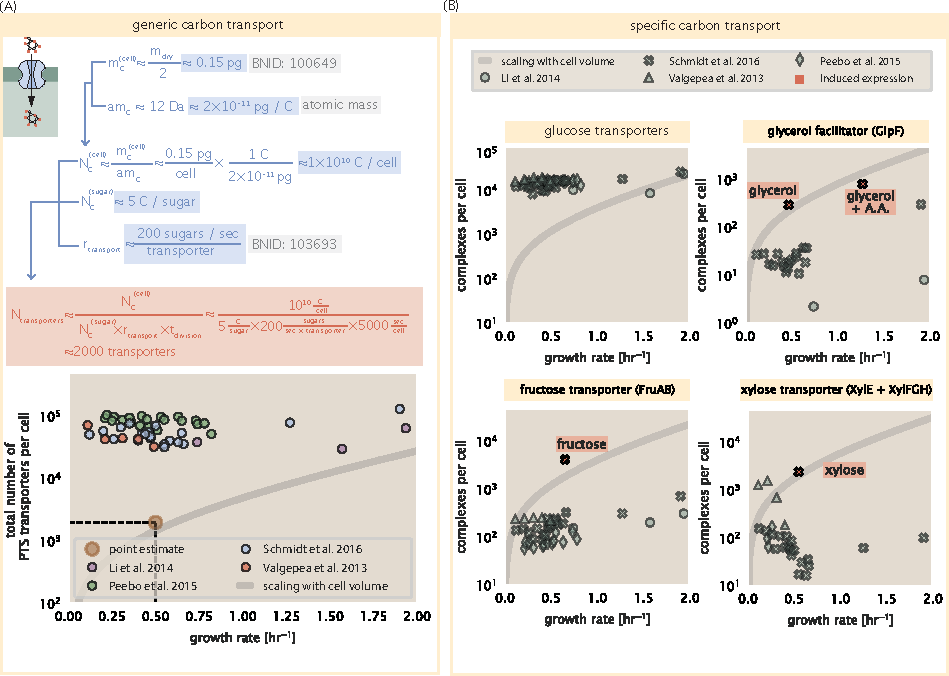
\includegraphics{main_figs/fig2_carbon_transport.pdf}
    \caption{\textbf{The abundance of carbon transport systems across growth
    rates.} (A) A simple estimate for the minimum number of generic carbohydrate
    transport systems (top) assumes $\approx 10^{10}$ C are needed to complete
    division, each transported sugar contains $\approx 6$ C, and each
    transporter conducts sugar molecules at a rate of $\approx 200$ per second.
    Bottom plot shows the estimated number of transporters needed at a growth
    rate of $\approx 0.5 $ per hr (light-brown point and dashed lines).  Colored
    points correspond to the mean number of PTS system sugar transporters
    (complexes annotated with the Gene Ontology term GO:0009401) for
    different growth conditions across different published datasets. (B) The
    abundance of various specific carbon transport systems plotted as a function
    of the population growth rate. The rates of substrate transport to compute
    the continuum growth rate estimate (grey line) were 200 glucose$\cdot$
    s$^{-1}$ (BNID: 103693, \cite{milo2010}),  2000 glycerol$\cdot$s$^{-1}$
    \citep{lu2003}, 200 fructose$\cdot$
    s$^{-1}$ (assumed to be similar to PtsI, BNID: 103693, \cite{milo2010}), and 50 xylose$\cdot$s$^{-1}$
    (assumed to be comparable to LacY, BNID:103159, \cite{milo2010}).
    Red points and highlighted text indicate conditions in
    which the
    only source of carbon in the growth medium induces expression of the
    transport system. Grey line in (A) and (B) represents the estimated number of transporters per cell at a continuum
    of growth rates.}
    \label{fig:carbon_tport}
    }
    \end{fullwidth}
\end{figure}

The estimate presented in \FIG{carbon_tport}(A) neglects any specifics of the
regulation of the carbon transport system and presents a  view of how
many carbohydrate transporters are present on average. Using the diverse array
of growth conditions explored in the proteomic data sets, we can explore how
individual carbon transport systems depend on the population growth rate. In
\FIG{carbon_tport}(B), we show the total number of carbohydrate transporters
specific to different carbon sources. A striking observation, shown in the
top-left plot of \FIG{carbon_tport}(B), is the constancy in the expression of the
glucose-specific transport systems. Additionally, we note that the total number
of glucose-specific transporters is tightly distributed at $\approx 10^4$ per cell,
the approximate number of transporters needed to sustain rapid growth of several
divisions per hour. This
illustrates that \textit{E. coli} maintains a substantial number of complexes
present for transporting glucose regardless of growth rate, which is known to be the preferential carbon
source \citep{monod1947, liu2005a, aidelberg2014}.

It is now understood that a large number of metabolic operons are regulated
with dual-input logic gates that are only expressed when glucose
concentrations are low (mediated by cyclic-AMP receptor protein CRP) and the
concentration of other carbon sources are elevated \citep{gama-castro2016, zhang2014a}. A
famed example of such dual-input regulatory logic is in the regulation of the
\textit{lac} operon which is only natively activated in the absence of glucose and the
presence of allolactose, an intermediate in lactose metabolism \citep{jacob1961}, though
we now know of many other such examples \citep{ireland2020, gama-castro2016,
belliveau2018}. This illustrates that once glucose is depleted from the
environment, cells have a means to dramatically increase the abundance of the
specific transporter needed to digest the next sugar that is present. Several
examples of induced expression of specific carbon-source transporters are
shown in \FIG{carbon_tport}(B). Points colored in red (labeled by red
text-boxes) correspond to growth conditions in which the specific carbon source
(glycerol, xylose, or fructose) is present. These plots show that, in the
absence of the particular carbon source, expression of the transporters is
maintained on the order of $\sim 10^2$ per cell. However, when the transport
substrate is present, expression is induced and the
transporters become highly-expressed. The grey lines in \FIG{carbon_tport}(B)
show the estimated number of transporters needed at each growth rate to satisfy
the cellular carbon requirement. It is notable that  in all cases, the magnitude
of induced expression (shown in red) falls close to the estimate, illustrating
the ability of the cell to tune expression in response to changing environments. Together, this generic estimation and the specific
examples of induced expression suggest that transport of carbon across the cell
membrane, while critical for growth, is not the rate-limiting step of cell division.

\subsection{Phosphorus and Sulfur Transport}
We now turn our attention towards other essential elements, namely phosphorus and
sulfur. Phosphorus is critical to the cellular energy economy in the form of
high-energy phosphodiester bonds making up DNA, RNA, and the NTP energy pool as
well as playing a critical role in the post-translational modification of
proteins and defining the polar-heads of lipids. In total, phosphorus
makes up $\approx$3\% of the cellular dry mass which in typical experimental conditions is in the form of inorganic phosphate. The cell membrane
has remarkably low permeability to this highly-charged and critical molecule,
therefore requiring the expression of active transport systems. In \textit{E. coli}, the proton
electrochemical gradient across the inner membrane is leveraged to transport
inorganic phosphate into the cell \citep{rosenberg1977}.
Proton-solute symporters are widespread in \textit{E. coli} \citep{ramos1977,
booth1979} and can have rapid transport rates of 50 to 100 molecules per second for
sugars and other solutes (BNID: 103159; 111777, \cite{milo2010}). As a more
extreme example, the proton transporters in the F$_1$-F$_0$ ATP synthase, which
use the proton electrochemical gradient for rotational motion, can shuttle
protons across the membrane at a rate of $\approx$ 1000 per second (BNID:
104890; 103390, \citep{milo2010}). In \textit{E.
coli} the PitA phosphate transport system has been shown to be very tightly coupled
with the proton electrochemical gradient with a 1:1 proton:phosphate
stoichiometric ratio \citep{harris2001, feist2007}. Taking the geometric mean of
the aforementioned estimates gives a plausible rate of phosphate transport on
the order of 300  per second. Illustrated in
\FIG{phospho_sulfo_tport}(A), we can estimate that $\approx$ 150
phosphate transporters are necessary to maintain an $\approx$ 3\% dry mass with
a 5000 s division time. This estimate is consistent with observation when we examine the
observed copy numbers of PitA in proteomic data sets (plot in
\FIG{phospho_sulfo_tport}(A)). While our estimate is very much in line with the
observed numbers, we emphasize that this is likely a slight overestimate of the
number of transporters needed as there are other phosphorous scavenging systems,
such as the ATP-dependent phosphate transporter Pst system which we have neglected.

Satisfied that there are a sufficient number of phosphate transporters
present in the cell, we now turn to sulfur transport as another potentially rate
limiting process. Similar to phosphate, sulfate is  highly-charged
and not particularly membrane permeable, requiring active
transport. While there exists a H+/sulfate symporter in \textit{E.
coli}, it is in relatively low abundance and is not well characterized
\citep{zhang2014}. Sulfate is predominantly acquired via the ATP-dependent ABC
transporter CysUWA system which also plays an important role in selenium
transport \citep{sekowska2000, sirko1995}. While specific kinetic details of
this transport system are not readily available, generic ATP transport
systems in prokaryotes transport on the order of 1 to 10 molecules per second
(BNID: 109035, \cite{milo2010}). Combining this generic
transport rate, measurement of sulfur comprising 1\% of dry mass, and a 5000
second division time yields an estimate of $\approx$ 1000 CysUWA
complexes per cell (\FIG{phospho_sulfo_tport}(B)). Once again, this estimate
is in notable agreement with proteomic data sets, suggesting that there are
sufficient transporters present to acquire the necessary sulfur. In a similar
spirit of our estimate of phosphorus transport, we emphasize that this is
likely an overestimate of the number of necessary transporters as we have
neglected other sulfur scavenging systems that are in lower abundance.


\begin{figure*}
    \begin{fullwidth}
    \centering{
        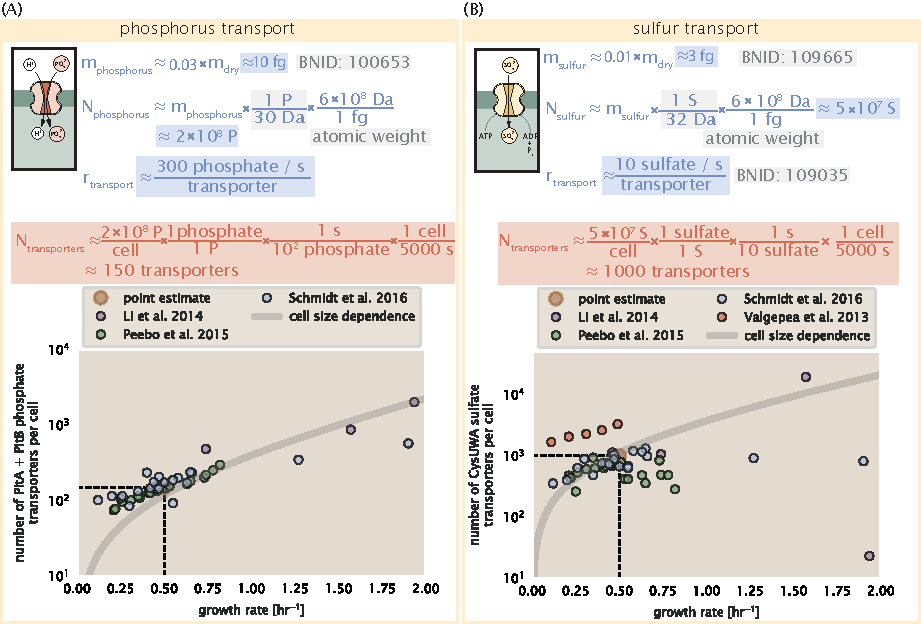
\includegraphics{main_figs/fig3_phospho_sulfo_transport.pdf}
        \caption{\textbf{Estimates and measurements of phosphate and sulfate
        transport systems as a function of growth rate.} (A) Estimate for the
        number of PitA phosphate transport systems needed to maintain a 3\%
        phosphorus \textit{E. coli} dry mass. Points in plot correspond to
        the the total number of PitA transporters per cell. (B) Estimate of
        the number of CysUWA complexes necessary to maintain a 1\% sulfur
        \textit{E. coli} dry mass. Points in plot correspond to average
        number of CysUWA transporter complexes that can be formed given the
        transporter stoichiometry [CysA]$_2$[CysU][CysW][Sbp/CysP]. Grey line
        in (A) and (B) represents the estimated number of transporters per
        cell at a continuum of growth rates.}
        \label{fig:phospho_sulfo_tport}
    }
    \end{fullwidth}
\end{figure*}


\subsection{Limits on Transporter Expression}
So which, if any, of these processes may be rate limiting for growth? As
suggested by \FIG{carbon_tport} (B), induced expression can lead to an
order-of-magnitude (or more) increase in the amount of transporters needed to
facilitate transport. Thus, if acquisition of nutrients was the limiting state
in cell division, could expression simply be increased to accommodate faster
growth? A way to approach this question is to compute the amount of space in the
bacterial membrane that could be occupied by nutrient transporters. Considering a rule-of-thumb for the surface area of
\textit{E. coli} of about 6 \textmu m$^2$ (BNID: 101792, \cite{milo2010}), we expect
an areal density for 1000 transporters to be approximately 200
transporters/ \textmu m$^2$. For a typical transporter occupying about 50
nm$^2$/dimer, this amounts to about only 1 percent of the total inner membrane
\citep{szenk2017}. In addition, bacterial cell membranes typically have
densities of 10$^5$ proteins/$\mu m^2$ \citep{phillips2018}, implying that the
cell could accommodate more transporters of a variety of species if it were rate
limiting. As we will see in the next section, however, occupancy of the membrane can
impose other limits on the rate of energy production.

\section{Cell Envelope Biogenesis}
In contrast to nutrient transporters, which support the synthesis of
biomolecules throughout the cell and therefore need to scale with the cell
size, here we must consider the synthesis of components that will need to
scale with the surface area of the cell. \textit{E. coli} is a rod-shaped
bacterium with a remarkably robust length-to-width aspect ratio of $\approx$
4:1 \citep{harris2018, ojkic2019}. Assuming this surface area is
approximately the same between the inner and outer membranes of \textit{E.
coli}, and the fact that each membrane is itself is a lipid bilayer (or, a
bilayer with lipopolysaccharides decorating the outer membrane), our rule-of-thumb
of 5 \textmu m$^2$ per surface suggests a total membrane surface area of
$\approx 20 $\textmu m$^2$ (see the Appendix Section "Estimation of Cell Size and Surface Area" for a description of the calculation of cell
surface area as a function of cell size). In this section, we will estimate
the number of key protein complexes needed to synthesize the lipids as well
as the complexes involved in assembling the peptidoglycan scaffold that make
up the cell envelope.

\subsection{Lipid Synthesis}
The dense packing of the membrane with proteins means that the cell membranes
are not composed entirely of lipid molecules, with only $\approx$ 40 \% of the
membrane area occupied by lipids or lipopolysaccharide, both of which have fatty
acid chains of similar length (BNID: 100078). Using a rule-of-thumb of 0.5
nm$^2$ as the surface area of the typical lipid (BNID: 106993), we can
estimate $\sim$ 2 $\times$ 10$^7$ lipids per cell, which is in close
agreement with experimental measurements (BNID: 100071, 102996).

The membranes of \textit{E. coli} are composed of a variety of different lipids,
each of which are unique in their structures and biosynthetic pathways
\citep{sohlenkamp2016}. Recently, a combination of stochastic kinetic modeling
\citep{ruppe2018} and \textit{in vitro} kinetic measurements
\citep{ranganathan2012, yu2011} has revealed remarkably slow steps in the fatty
acid synthesis pathways which may serve as the rate limiting reactions for
making new membrane fatty acids (that become components of a variety of
membrane lipids) in \textit{E. coli}. One such step is the removal of hydroxyl
groups from the fatty-acid chain by ACP dehydratase that leads to the formation
of carbon-carbon double bonds. This reaction, catalyzed by proteins FabZ and
FabA \citep{yu2011}, have been estimated to have kinetic
turnover rates of $\approx$ 1 dehydration per second per enzyme
\citep{ruppe2018}. Thus, given this rate and the need to synthesize $\approx$ 2
$\times$ 10$^7$ lipids over 5000 seconds, one can estimate that a typical cell
requires $\approx$ 4000 ACP dehydratases. This is in reasonable agreement with
the experimentally observed copy numbers of FabZ and FabA
(\FIG{cell_envelope}(A)). Furthermore, we can extend this estimate to account
for the change in membrane surface area as a function of the growth rate (grey
line in \FIG{cell_envelope}(A)), which captures the observed growth rate
dependent expression of these two enzymes.

\subsection{Peptidoglycan Synthesis}
The exquisite control of bacteria over their cell shape is due primarily to a stiff, several nanometer thick meshwork of
polymerized discaccharides that makes up the cell wall termed the peptidoglycan. The formation of the peptidoglycan is an intricate
process involving many macromolecular players \citep{shi2018, morgenstein2015},
whose coordinated action synthesizes the individual subunits and integrates them
into the peptidodglycan network which maintains cell shape and integrity even in the face of
large-scale perturbations \citep{harris2018,shi2018}.
Due to the extensive degree of chemical crosslinks between glycan strands, the
entire peptidoglycan is a single molecule comprising $\approx$ 3\% of the cellular dry mass (BNID:
1019360), making it the most massive molecule in \textit{E. coli}. The
polymerized unit of the peptidoglycan is a N-acetylglucosamine and
N-acetylmuramic acid disaccharide, of which the former is functionalized with a
short pentapeptide. With a mass of $\approx$ 1000 Da, this unit, which we refer
to as a murein subunit, is polymerized to form long strands in the periplasm
which are then attached to each other via their peptide linkers. Together, these
quantities provide an estimate of $\approx$ 5 $\times$ 10$^6$ murein subunits
per cell.

There are various steps which one could consider \textit{a priori} to be a
limiting process in the synthesis of peptidoglycan, including the
biosynthesis steps that occur in the cytoplasm, the transglycosylation
reaction which adds new subunits to the glycan filaments, and the formation
of the peptide crosslinks between strands
\cite{shi2018,morgenstein2015,lovering2012,barreteau2008}. Despite the
extensive mechanistic characterization of these components,
\textit{quantitative} characterization of the individual reaction rates along
the entire kinetic pathway of remain scarce and make identification of any
particularly slow steps difficult. However, such measurements have recently
been made for the crosslinking machinery (transpeptidases,
\cite{catherwood2020}) of the peptodioglycan which provides lateral
structural integrity to the peptidoglycan shell. As the primary mechanism of
subunit integration occurs by a complex with both transglycosylation and
transpeptidation activities \cite{shi2018} and that the measured turnover of
transpeptidases being rather slow ($\approx$ 2 crosslinking reactions per
second) we therefore consider only the transpeptidation reaction in this
work. We believe that, in lieu of other quantitative measurements,
crosslinking represents a reasonable candidate for a rate-limiting step in
growth as it is required for cell size and shape homeostasis.

In principle, each murein subunit can be involved in such a crosslink. In
some microbes, such as in gram-positive bacterium \textit{Staphylococcus
aureus}, the extent of crosslinking can be large with $>$ 90\% of
pentapeptides forming a connection between glycan strands. In \textit{E.
coli}, however, a much smaller proportion ($\approx$ 20\%) of the peptides
are crosslinked, resulting in a weaker and more porous cell wall
\citep{vollmer2008a, rogers1980}. The formation of these crosslinks occurs
primarily during the polymerization of the murein subunits and is facilitated
by a family of transpeptidase enzymes. The four primary transpeptidases of
\textit{E. coli} have only recently been quantitatively characterized
\textit{in vivo}, via liquid chromatography mass spectrometry, which revealed
a notably slow kinetic turnover rate of $\approx 2$ crosslinking reactions
formed per second per enzyme \citep{catherwood2020}.

Assembling these quantities permits us to make an estimate that on the order
of $\approx$ 100 transpeptidases per cell are needed for complete maturation
of the peptidoglycan, given a division time of $\approx$ 5000 seconds; a
value that is comparable to experimental observations
[\FIG{cell_envelope}(B)]. Expanding this estimate to account for the changing
mass of the peptidoglycan as a function of growth rate [grey line in
\FIG{cell_envelope}(B)] predicts an order-of-magnitude increase in the
abundance of the transpeptidases when the grow rate is increased by a factor
of four. However, it is difficult to compare this to the observed complex
abundances as systematic disagreements between the different data obfuscates
any significant dependence on growth rate.

\subsubsection{Limits on Cell Wall Biogenesis}
While the processes we have considered represent only a small portion of
proteins devoted to cell envelope biogenesis, we find it unlikely that they
limit cellular growth in general. The relative amount of mass required for
lipid and peptidoglycan components decrease at faster growth rates due to a
decrease in their surface area to volume (S/V) ratio \citep{ojkic2019}.
Furthermore, despite the slow catalytic rate of FabZ and FabA in lipid
synthesis, experimental data and recent computational modeling has shown that
the rate of fatty-acid synthesis can be drastically increased by increasing
the concentration of FabZ \citep{yu2011, ruppe2018}. With a proteome size of
$\approx$ 3$\times$10$^6$ proteins, a hypothetical 10-fold increase in
expression from 4000 to 40,000 ACP dehydratases would result in a paltry
$\approx$ 1\% increase in the size of the proteome. In the context of
peptidoglycan synthesis, we note that our estimate considers only the
transpeptidase enzymes that are involved in lateral and longitudinal elongation
of the peptidoglycan. This neglects the presence of other transpeptidases
that are present in the periplasm and also involved in remodeling and
maturation of the peptidoglycan. It is therefore possible that if this was
setting the speed limit for cell division, the simple expression of more
transpeptidases may be sufficient to maintain the structural integrity of the
cell wall.

\begin{figure}
    \begin{fullwidth}
    \centering{
    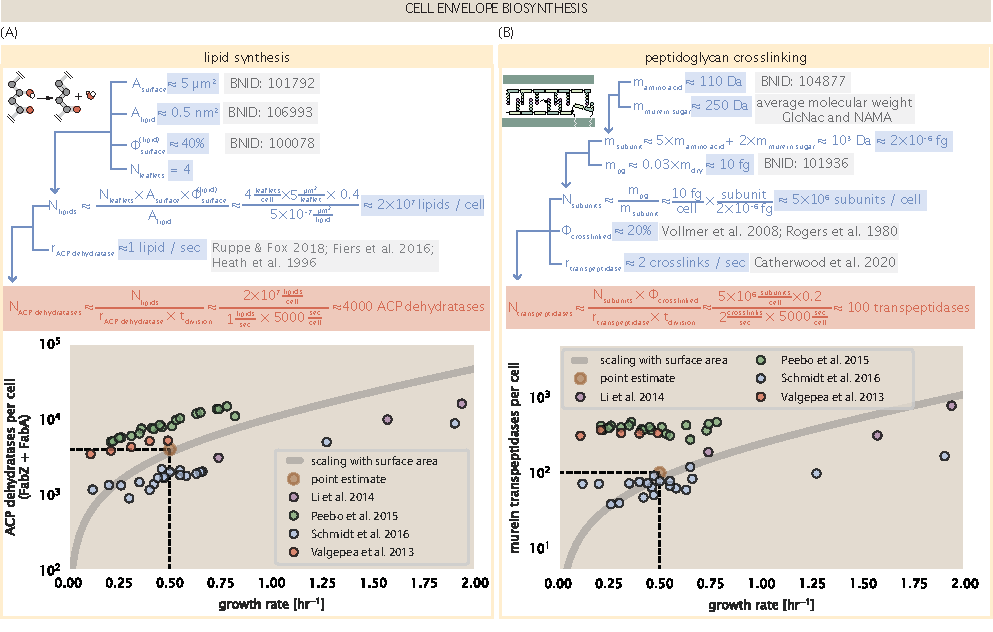
\includegraphics{main_figs/fig3_cell_wall_peptidoglycan.pdf}
    \caption{(A) Top panel shows an estimation for the
            number of ACP dehydratases necessary to form functional
            phospholipids, which is assumed to be a rate-limiting step on
            lipid synthesis. The rate of ACP dehydratases was inferred from
            experimental measurements via a stochastic kinetic model
            described in \cite{ruppe2018}. Bottom panel shows the
            experimentally observed complex copy numbers using the
            stoichiometries [FabA]$_2$ and [FabZ]$_2$. (B) An estimate for
            the number of peptidoglycan transpeptidases needed to complete
            maturation of the peptidoglycan. The mass of the murein subunit
            was estimated by approximating each amino acid in the
            pentapeptide chain as having a mass of 110 Da and each sugar in
            the disaccharide having a mass of $\approx$ 250 Da. The
            \textit{in vivo} rate of transpeptidation in \textit{E. coli}
            was taken from recent analysis by \cite{catherwood2020}. The
            bottom panel shows experimental measurements of the
            transpeptidase complexes in \textit{E. coli} following the
            stoichiometries [MrcA]$_2$, [MrcB]$_2$, [MrdA]$_1$, and
            [MrdB]$_1$. Grey curves in each plot show the estimated number of
            complexes needed to satisfy the synthesis requirements scaled by
            the surface area as a function of growth
            rate.}
            \label{fig:cell_envelope}
    }
    \end{fullwidth}
\end{figure}

\section{Energy Production}
Cells consume and generate energy predominantly in the form of nucleoside
triphosphates (NTPs) in order to grow. The high-energy phosophodiester bonds of
(primarily) ATP power a variety of cellular processes that drive biological
systems away from thermodynamic equilibrium. We now turn to the synthesis of ATP
as a potential process that may limit growth, which also requires us to consider
the maintenance of the electrochemical proton gradient which powers it.

\subsection{ATP Synthesis}
Hydrolysis of the terminal phosphodiester bond of ATP into ADP (or
alternatively GTP and GDP) and an inorganic phosphate provides the
thermodynamic driving force in a wide array of biochemical reactions. One
such reaction is the formation of peptide bonds during translation, which
requires $\approx$ 2 ATPs for the charging of an amino acid to the tRNA and
$\approx$ 2 GTPs for the formation of each peptide bond. Assuming the ATP
costs associated with error correction and post-translational modifications
of proteins are negligible, we can make the approximation that each peptide
bond has a net cost of $\approx$ 4 ATP (BNID: 101442).
Formation of GTP from ATP is achieved via the action of nucleoside
diphosphate kinase, which catalyzes this reaction without an energy
investment \citep{lascu2000} and therefore consider all NTP requirements of
the cell to be functionally equivalent to being exclusively ATP. In total,
the energetic costs of peptide bond formation consume $\approx$ 80\% of the
cells ATP budget [BNID: 107782; 106158; 101637; 111918,
\cite{lynch2015,stouthamer1973}]. The pool of ATP is produced by the
F$_1$-F$_0$ ATP synthase -- a membrane-bound rotary motor which under ideal
conditions can yield $\approx$ 300 ATP per second [BNID: 114701;
\cite{weber2003}].

To estimate the total number of ATP equivalents consumed during a cell cycle, we
will make the approximation that there are $\approx 3\times10^6$ proteins per
cell with an average protein length of $\approx$ 300 peptide bonds (BNID:
115702; 108986; 104877). Taking these values together, coupled with an estimate
of $\approx$ 4 ATP equivalents per peptide bond, we find that the typical
\textit{E. coli} cell consumes $\sim 5 \times 10^9$ ATP per cell cycle on
protein synthesis alone. Assuming that each ATP synthases operates at its
maximal speed (300 ATP per second per synthase), $\approx$ 3000 ATP synthases
are needed to keep up with the energy demands of the cell. This estimate
is comparable with the experimental observations,  shown in
\FIG{energy_production} (A). We note that this estimate assumes all ATP is
synthesized via ATP synthase and neglects synthesis via fermentative metabolism.
This simplification may explain why at the fastest growth rates ($\approx$ 2
hr$^{-1}$), our continuum estimate predicts more synthase than is experimentally
observed (gray line in \FIG{energy_production}). At rapid growth rates,
\textit{E. coli} enters a type of overflow metabolism where fermentative
metabolism becomes pronounced \citep{szenk2017}.

\subsection{Generating the Proton Electrochemical Gradient}
In order to produce ATP, the F$_1$-F$_0$ ATP synthase itself must consume
energy. Rather than burning through its own product (and violating
thermodynamics), this intricate macromolecular machine has evolved to exploit
the electrochemical potential established across the inner membrane through
cellular respiration. This electrochemical gradient is manifest by the pumping
of protons into the intermembrane space via the electron transport chains as
they reduce NADH. In \textit{E. coli}, this potential difference is $\approx
-$200 mV (BNID: 102120). A simple estimate of the inner membrane as a capacitor
with a working voltage of -200 mV reveals that $\approx 2\times 10^4$ protons
must be present in the intermembrane space. However, each rotation of an ATP
synthase shuttles $\approx$ 4 protons into the cytosol (BNID: 103390). With a few thousand ATP
synthases producing ATP at their maximal rate, the potential difference would be
rapidly abolished in a few milliseconds if it were not being actively
maintained.

The electrochemistry of the electron transport complexes of \textit{E. coli}
have been the subject of intense biochemical and biophysical study
\citep{ingledew1984, khademian2017,cox1970,henkel2014}. A recent work
\citep{szenk2017} examined the respiratory capacity of the \textit{E. coli}
electron transport complexes using structural and biochemical data, revealing
that each electron transport chain rapidly pumps protons into the
intermembrane space at a rate of $\approx$ 1500 protons per second (BIND:
114704; 114687). Using our estimate of the number of ATP synthases required
per cell [\FIG{energy_production}(A)], coupled with these recent
measurements, we estimate that $\approx 3000$ electron transport complexes
would be necessary to facilitate the $\sim 5 \times 10^6$ protons per second
diet of the cellular ATP synthases. This estimate is in agreement with the
number of complexes identified in the proteomic datasets [plot in
\FIG{energy_production}(B)]. This suggests that every ATP synthase must be
accompanied by $\approx$ 1 functional electron transport chain.

\begin{figure}
    \begin{fullwidth}
        \centering{
            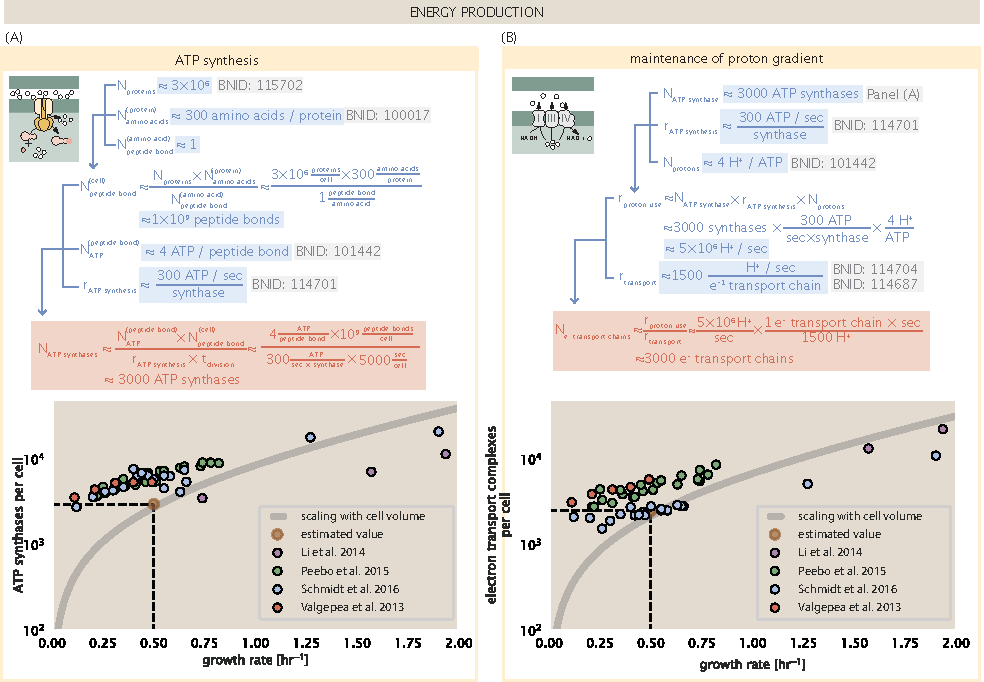
\includegraphics{main_figs/fig4_energy_production.pdf}
            \caption{\textbf{The abundance of F$_1$-F$_0$ ATP synthases and
            electron transport chain complexes as a function of growth
            rate.} (A) Estimate of the number of F$_1$-F$_0$ ATP synthase
            complexes needed to accommodate peptide bond formation and other NTP
            dependent processes. Points in plot correspond to the
            mean number of complete F$_1$-F$_0$ ATP synthase complexes that
            can be formed given proteomic measurements and the subunit
            stoichiometry
            [AtpE]$_{10}$[AtpF]$_2$[AtpB][AtpC][AtpH][AtpA]$_{3}$[AtpG][AtpD]$_3$.
            (B) Estimate of the number of electron transport chain complexes
            needed to maintain a membrane potential of $-$200 mV given
            estimate of number of F$_1$-F$_0$ ATP synthases from (A). Points
            in plot correspond to the average number of complexes identified
            as being involved in aerobic respiration by the Gene Ontology
            identifier GO:0019646 that could be formed given proteomic
            observations. These complexes include cytochromes \textit{bd1}
            ([CydA][CydB][CydX][CydH]), \textit{bdII} ([AppC][AppB]),
            \textit{bo$_3$},([CyoD][CyoA][CyoB][CyoC]) and NADH:quinone
            oxioreducase I
            ([NuoA][NuoH][NuoJ][NuoK][NuoL][NuoM][NuoN][NuoB][NuoC][NuoE][NuoF][NuoG][NuoI])
            and II ([Ndh]). Grey lines in both (A) and (B) correspond to the
            estimate procedure described, but applied to a continuum of growth
            rates. We direct the reader to the Supporting Information for a more
            thorough description of this approach.}
        \label{fig:energy_production}
        }
    \end{fullwidth}
\end{figure}


\subsubsection{Limits on Biosynthesis in a Crowded Membrane}
Our estimates thus far have focused on biochemistry at the periphery of the cell.
Since surface area and volume do not scale identically as cell size changes,  in
order to better understand the physical constraints on transport and  energy
production it is necessary to consider the consequence of a changing S/V
ratio, which will decrease at faster growth rates. Here we use our analysis of
ATP production  to consider this constraint.

In our estimate of ATP production above we found that a cell demands about $5
\times 10^9$ ATP per cell cycle or $10^6$ ATP/s. With a cell volume of roughly 1
fL (BNID: 100004), this corresponds to about $2 \times 10^{10}$ ATP per fL of cell volume, in
line with previous estimates \citep{stouthamer1977, szenk2017}. In
\FIG{energy_scaling} (A) we plot this ATP demand as a function of the S/V ratio
in green, where we have considered a range of cell shapes from spherical to
rod-shaped with an aspect ratio (length/width) equal to 4. In order to consider
the maximum ATP that could be produced, we consider the amount of ATP that can
be generated by a membrane filled with ATP synthase and electron transport
complexes and a maximal production rate of about 3 ATP / (nm$^2 \cdot$s)
\citep{szenk2017}. This is shown in blue in \FIG{energy_scaling}(A), which shows
that at least for the growth rates observed (right column in plot), the energy
demand is roughly an order of magnitude less. Interestingly, \cite{szenk2017}
found that ATP production by respiration is less efficient than by
fermentation on a per membrane area basis, due to the additional proteins of the
electron transport chain. This suggests that, even under anaerobic growth, cells
will have sufficient membrane space for ATP production.

The analysis highlights that there will indeed be a maximum attainable cell size
due to a diminishing capacity to provide resources as the cell increases in
size. The maximum energy production in \FIG{energy_scaling}(A), however, does
represent a somewhat unachievable limit since the inner membrane must also
include other proteins such as those we've considered for nutrient transport and cell
wall biogenesis. To better understand the overall proteomic makeup of the inner
membrane, we therefore used Gene Ontology (GO) annotations \citep{ashburner2000,
thegeneOntologyconsortium2018} to identify all proteins embedded or peripheral
to the inner membrane (GO term: 0005886). Those associated but not
membrane-bound include proteins like MreB and FtsZ and must nonetheless be
considered as a vital component occupying space on the membrane. In
\FIG{energy_scaling}(B), we find that the total protein mass per \textmu m$^2$
is nearly constant across growth rates. Interestingly, when we consider the
distribution of proteins grouped by their Clusters of Orthologous Groups (COG)
\citep{tatusov2000}, the relative abundance for those in metabolism (including
ATP synthesis via respiration) is also relatively constant across growth rates,
suggesting that no one process (energy production, nutrient uptake, etc.) is
particularly dominating even at fast growth rates [\FIG{energy_scaling}(C)].

\begin{figure}
    \begin{fullwidth}
        \centering{
            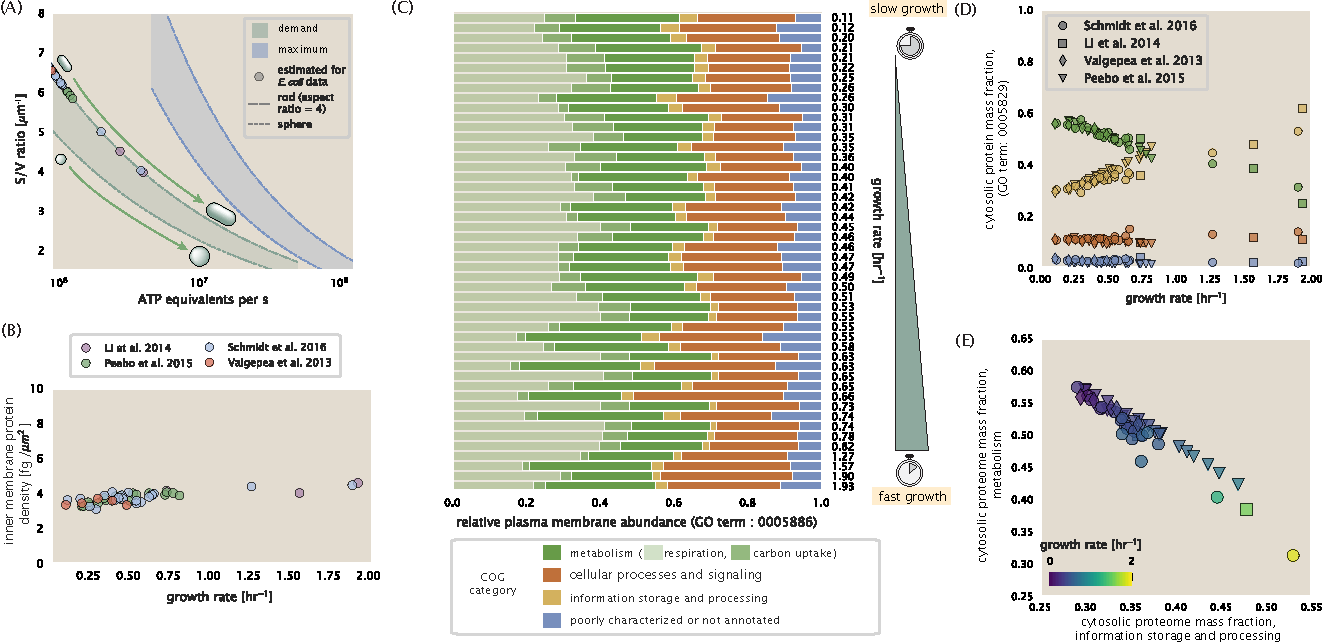
\includegraphics{main_figs/fig5_energy_SV_scaling.pdf}
            \caption{\textbf{Influence of cell size and surface area to volume
            (S/V) ratio on ATP production and inner membrane composition.} (A) Scaling
            of ATP demand and maximum ATP production through respiration as a
            function of S/V ratio. Cell volumes of 0.5 fL to 50 fL were
            considered, with the dashed (\texttt{- -}) line corresponding to a
            sphere and the dash-dot line (\texttt{-.}) reflecting a rod-shaped
            bacterium like \textit{E. coli} with a typical aspect ratio (length
            / width) of 4 \citep{shi2018}. The ATP demand is calculated as
            $10^6$ ATP/(\textmu m$^3$ s), while the maximum ATP production rate
            is taken to be 3 ATP / (nm$^2 \cdot$s)
            \citep{szenk2017}, with calculations of \textit{E. coli} volume and
            surface area detailed in Appendix \nameref{sec:protein_size_SV}. In
            this calculation, 50\% of the bacterial inner membrane is assumed to
            be protein, with the remainder lipid. (B) Total protein mass per
            \textmu m$^2$ calculated for proteins with inner membrane annotation
            (GO term: 0005886). (C) Relative protein abundances by mass based on
            COG annotation. Metabolic proteins are further separated into
            respiration (F$_1$-F$_0$ ATP synthase, NADH dehydrogenase I,
            succinate:quinone oxidoreductase, cytochrome bo$_3$ ubiquinol
            oxidase, cytochrome bd-I ubiquinol oxidase) and carbohydrate
            transport (GO term: GO:0008643). Note that the elongation factor
            EF-Tu can also associate with the inner membrane, but was excluded
            in this analysis due to its high relative abundance (roughly
            identical to the summed protein shown in part
            (B)).}\label{fig:energy_scaling}
            }
                \end{fullwidth}
\end{figure}

\section{Processes of the Central Dogma}
Up to this point, we have considered a variety of transport and biosynthetic
processes that are critical to acquiring and generating new cell mass. While
there are of course many other metabolic processes we could consider, we now
turn our focus to some of the most important processes which \textit{must} be
undertaken irrespective of the growth conditions -- those of the central
dogma.

\subsection{DNA Replication}
Most bacteria (including \textit{E. coli}) harbor a single, circular chromosome
and can have extra-chromosomal plasmids up to $\sim$ 100 kbp in length. While
we consider the starting material dNTPs in \FIGSUPP[DNA_synthesis]{dntp} and
discussed further in the Appendix Section "\nameref{sec:SI_central_dogma}", here we focus
our quantitative thinking on the chromosome of \textit{E. coli}, which
harbors $\approx$ 5000 genes and $\approx 5\times 10^6$ base pairs.

To successfully divide and produce viable progeny, this chromosome must be
faithfully replicated and segregated into each nascent cell. Replication is
initiated at a single region of the chromosome termed the \textit{oriC} locus
where a pair of replisomes, each consisting of two DNA polymerase III,
begin their high-fidelity replication of the genome in opposite directions
\citep{fijalkowska2012}. \textit{In vitro} measurements have shown that DNA
Polymerase III copies DNA at a rate of $\approx 600$ nucleotides per second
(BNID: 104120). Therefore, to replicate a single chromosome, two replisomes
moving at their maximal rate would copy the entire genome in $\approx$ 4000
s. Thus, with a division time of 5000 seconds, there is sufficient time for a pair
of replisomes complexes to replicate the entire genome.

\begin{figure}
  \centering{
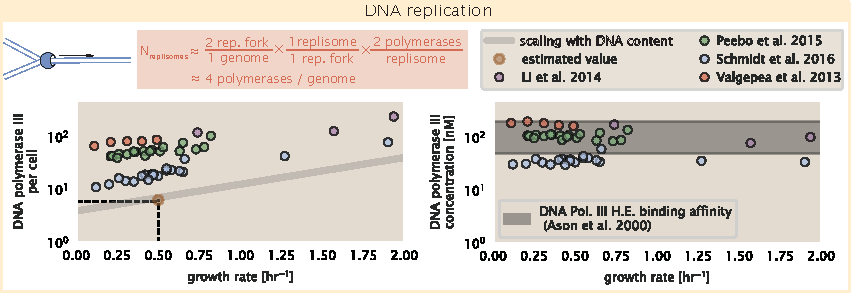
\includegraphics{main_figs/fig6_DNA_replication_main.pdf}
\caption{\textbf{Complex abundance estimates for dNTP synthesis and DNA
replication.} An estimate
for the minimum number of DNA polymerase holoenzyme complexes needed to
facilitate replication of a single genome. Points in the left-hand plot correspond
to the total number of DNA polymerase III holoenzyme complexes
([DnaE]$_3$[DnaQ]$_3$[HolE]$_3$[DnaX]$_5$[HolB][HolA][DnaN]$_4$[HolC]$_4$[HolD]$_4$)
per cell. Right-hand plot shows the effective concentration of DNA polymerase III
holoenzyme (See Appendix \nameref{sec:protein_size_SV} for calculation of cell
size). Grey lines in left-hand panel show the estimated number of
complexes needed as a function of growth, the details of which are described
in the Supplemental Information.} \label{fig:DNA_synthesis}
 }
\figsupp[Estimate and observations of the abundance of ribonucleotide
reductase, a key component in dNTP synthesis.]{Estimate of the number of
ribonucleotide reductase enzymes needed to facilitate the synthesis of
$\approx 10^7$ dNTPs over the course of a 5000 second generation time. Points
in the plot correspond to the total number of ribonucleotide reductase I
([NrdA]$_2$[NrdB]$_2$) and ribonucleotide reductase II ([NrdE]$_2$[NrdF]$_2$)
complexes. Grey lines in top panel show the estimated number of complexes
needed as a function of growth, the details of which are described in the
Appendix.}{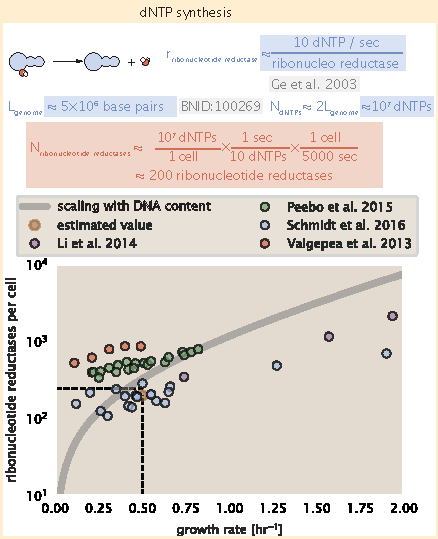
\includegraphics{main_figs/fig6-S1_dNTP_synthesis.pdf}}\label{figsupp:dntp}

\end{figure}

In rapidly growing cultures, bacteria like \textit{E. coli}
can initiate as many as 10 - 12 replication forks at a
given time \citep{bremer2008, si2017},  we expect only a few DNA polymerases
($\approx 10$) are needed. However, as shown in \FIG{DNA_synthesis}, DNA
polymerase III is nearly an order of magnitude more abundant. This discrepancy
can be understood by considering its binding constant to DNA. \textit{In vitro} characterization has quantified the $K_D$ of
DNA polymerase III holoenzyme to single-stranded and double-stranded DNA to be
50 and 200 nM, respectively \citep{ason2000}. The right-hand plot in
\FIG{DNA_synthesis} shows that the concentration of DNA polymerase III
across all data sets is within this range. Thus, its copy number appears to vary such that its
concentration is approximately equal to the dissociation constant to the DNA.
While the processes regulating the initiation of DNA replication are complex and
involve more than just the holoenzyme, these data indicate that the kinetics of
replication rather than the explicit copy number of the DNA polymerase III
holoenzyme is the more relevant feature of DNA replication to consider. In light
of this, the data in \FIG{DNA_synthesis} suggests that for bacteria like
\textit{E. coli}, DNA replication does not represent a rate-limiting step in
cell division. However, it is worth noting that for bacterium like \textit{C.
crescentus} whose chromosomal replication is initiated only once per cell cycle
\citep{jensen2001}, the time to double their chromosome indeed represents an
upper limit to their growth rate.

\subsection{RNA Synthesis}\label{sec:RNA_synthesis}
With the machinery governing the replication of the genome accounted for, we
now turn our attention to the next stage of the central dogma -- the
transcription of DNA to form RNA. We primarily consider three major groupings
of RNA, namely the RNA associated with ribosomes (rRNA), the RNA encoding the
amino-acid sequence of proteins (mRNA), and the RNA which links codon
sequence to amino-acid identity during translation (tRNA). Despite the varied
function of these RNA species, they share a commonality in that they are
transcribed from DNA via the action of RNA polymerase. In the coming
paragraphs, we will consider the synthesis of RNA as a rate limiting step in
bacterial division by estimating how many RNA polymerases must be present to
synthesize all necessary rRNA, mRNA, and tRNA.

\subsubsection{rRNA}
We begin with an estimation of the number of RNA polymerases needed to
synthesize the rRNA that serve as catalytic and structural elements of the
ribosome. Each ribosome contains three rRNA molecules of lengths 120, 1542,
and 2904 nucleotides (BNID: 108093, \cite{milo2010}), meaning each ribosome
contains $\approx$ 4500 nucleotides. As the \textit{E. coli} RNA polymerase
transcribes DNA to RNA at a rate of $\approx$ 40 nucleotides per second
(BNID: 101904, \cite{milo2010}), it takes a single RNA polymerase
$\approx$ 100 s to synthesize the RNA needed to form a single functional ribosome.
Therefore, in a 5000 s division time, a single RNA polymerase transcribing
rRNA at a time would result in only $\approx$ 50 functional ribosomal rRNA
units -- far below the observed number of $\approx 10^4$ ribosomes per cell.

Of course, there can be more than one RNA polymerase transcribing the rRNA genes
at any given time. To elucidate the \textit{maximum} number of rRNA units that can
be synthesized given a single copy of each rRNA gene, we will consider a
hypothesis in which the rRNA operon is completely tiled with RNA polymerase.
\textit{In vivo} measurements of the kinetics of rRNA transcription have revealed that
RNA polymerases are loaded onto the promoter of an rRNA gene at a rate of
$\approx$ 1 per second (BNID: 111997; 102362, \cite{milo2010}). If RNA
polymerases are being constantly loaded on to the rRNA genes at this rate,
then we can assume that $\approx$ 1 functional rRNA unit is
synthesized per second. With a 5000 second division time, this hypothesis
leads to a maximal value of 5000 functional rRNA units, still undershooting
the observed number of $10^4$ ribosomes per cell.

\textit{E. coli}, like many other bacterium, have evolved a clever mechanism to surpass this kinetic limit
for the rate of rRNA production. Rather than having only one copy of each rRNA
gene, \textit{E. coli} has seven copies of the operon (BIND: 100352,
\cite{milo2010}) four of which are localized directly adjacent to the origin of
replication \citep{birnbaum1971}. As fast growth also implies an increased gene
dosage due to paralellized chromosomal replication, the total number of rRNA
genes can be on the order of $\approx$ 10 -- 70 copies at moderate to fast
growth rates \citep{stevenson2004}. Using our standard time scale of a 5000
second division time, we can make the lower-bound estimate that the typical cell
will have 7 copies of the rRNA operon. Synthesizing one functional rRNA unit per
second per rRNA operon, a total of $4 \times 10^4$ rRNA units can be
synthesized, comfortably above the observed number of ribosomes per cell.

How many RNA polymerases are then needed to constantly transcribe 7 copies of
the rRNA genes? We approach this estimate by considering the maximum number
of RNA polymerases tiled along the rRNA genes with a loading rate of 1 per
second and a transcription rate of 40 nucleotides per second. Considering
that a RNA polymerase has a physical footprint of approximately 40
nucleotides (BNID: 107873, \cite{milo2010}), we can expect
$\approx$ 1 RNA polymerase per 80 nucleotides. With a total length of
$\approx$ 4500 nucleotides per operon and 7 operons per cell, the maximum
number of RNA polymerases that can be transcribing rRNA at any given time is
$\approx$ 400. As we will see in the coming sections, the
synthesis of rRNA is the dominant requirement of the RNA polymerase pool.

\subsubsection{mRNA}
To form a functional protein, all protein coding genes must first be
transcribed from DNA to form an mRNA molecule. While each protein requires an
mRNA blueprint, many copies of the protein can be synthesized from a single
mRNA. Factors such as strength of the ribosomal binding site, mRNA stability,
and rare codon usage frequency dictate the number of proteins that can be
made from a single mRNA, with yields ranging from 10$^1$ to 10$^4$ (BNID: 104186; 100196;
106254, \cite{milo2010}). Computing the geometric mean of this range yields
$\approx$ 1000 proteins synthesized per mRNA, a value that agrees with
experimental measurements of the number of proteins per cell ($\approx 3
\times 10^6$, BNID: 100088, \cite{milo2010}) and total number of mRNA per
cell ($\approx 3 \times 10^3$, BNID:100064, \cite{milo2010}).

This estimation captures the \textit{steady-state} mRNA copy number, meaning
that at any given time, there will exist approximately 3000 unique mRNA
molecules. To determine the \textit{total} number of mRNA that need to be
synthesized over the cell's lifetime, we must consider degradation of the mRNA.
In most bacteria, mRNAs are rather unstable with life times on the order of
several minutes (BNID: 104324; 106253; 111927; 111998, \cite{milo2010}). For
convenience, we assume that the typical mRNA in our cell of interest has a
typical lifetime of $\approx$ 300 seconds. Using this value, we can determine
the total mRNA production rate to maintain a steady-state copy number of 3000
mRNA per cell. While we direct the reader to the appendix for a more detailed
discussion of mRNA transcriptional dynamics, we state here that the total mRNA
production rate must be on the order of $\approx$ 15 mRNA per second. In
\textit{E. coli}, the average protein is $\approx$ 300 amino acids in length
(BNID: 108986; \cite{milo2010}), meaning that the corresponding mRNA is
$\approx$ 900 nucleotides which we will further approximate as $\approx$ 1000
nucleotides to account for the non-protein coding regions on the 5' and
3' ends. This means that the cell must have enough RNA polymerase molecules
about to sustain a transcription rate of $\approx 1.5 \times 10^4$ nucleotides
per second. Knowing that a single RNA polymerase polymerizes RNA at a clip of 40
nucleotides per second, we arrive at a comfortable estimate of $\approx$ 250 RNA
polymerase complexes needed to satisfy the mRNA demands of the cell. It is worth
noting that this number is approximately half of that required to synthesize
enough rRNA, as we saw in the previous section. We find this to be a striking
result as these 250 RNA polymerase molecules are responsible for the
transcription of the $\approx$ 4000 protein coding genes that are not ribosome
associated.

\subsubsection{tRNA}
The final class of RNA molecules worthy of quantitative consideration are the
tRNAs that are used during translation to map codon sequence on mRNA to specific amino acids.
Unlike mRNA or rRNA, each individual tRNA is remarkably short, ranging
from 70 to 95 nucleotides each (BNID: 109645; 102340, \cite{milo2010}). What
they lack in length, they make up for in abundance, with reported values ranging from
$\approx$6$\times$10$^4$ (BNID: 105280, \cite{milo2010}) to
$\approx$4$\times$10$^5$ (BNID: 108611). To test tRNA synthesis as a possible
growth-rate limiting stage, we will err towards a higher abundance of $\approx$
4$\times$10$^5$ per cell. Combining the abundance and tRNA length measurements,
we make the estimate that $\approx 5 \times 10^7$ nucleotides are sequestered in tRNA per cell.
Unlike mRNA, tRNA is remarkably stable with typical lifetimes \textit{in vivo}
on the order of $\approx$ 48 hours \citep{abelson1974,svenningsen2017} -- well
beyond the timescale of division. Once again using our rule-of-thumb for the
rate of transcription to be 40 nucleotides per second and assuming a division
time of $\approx$ 5000 seconds, we arrive at an estimate of $\approx$ 150 RNA
polymerases to synthesize enough tRNA. This requirement pales in comparison to
the number of polymerases needed to generate the rRNA and mRNA pools and can be
neglected as a significant transcriptional burden.

\begin{figure}
    \begin{fullwidth}
    \centering{
        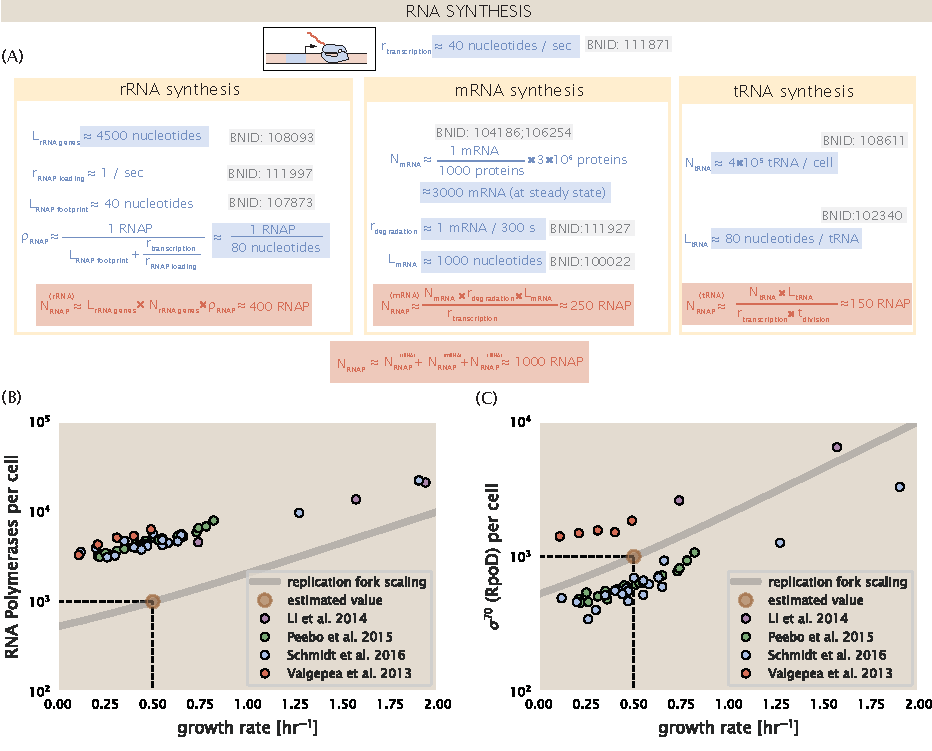
\includegraphics{main_figs/fig7_RNA_synthesis.pdf}
        \caption{\textbf{Estimation of the RNA polymerase demand and
        comparison with experimental data.} (A) Estimations for the number of
        RNA polymerase needed to synthesize sufficient quantities of rRNA, mRNA,
        and tRNA from left to right, respectively. Bionumber Identifiers (BNIDs)
        are provided for key quantities used in the estimates. (B) The RNA
        polymerase core enzyme copy number as a function of growth rate. Colored
        points correspond to the average number RNA polymerase core enzymes that
        could be formed given a subunit stoichiometry of [RpoA]$_2$[RpoC][RpoB].
        (C) The abundance of $\sigma^{70}$ as a function of growth rate.
        Estimated value for the number of RNAP is shown in (B) and (C) as a
        translucent brown point at a growth rate of 0.5 hr$^{-1}$.}
    \label{fig:RNA_synthesis}
    }
    \end{fullwidth}
\end{figure}


\subsubsection{RNA Polymerase and $\sigma$-factor Abundance}
These estimates, summarized in \FIG{RNA_synthesis} (A), reveal that synthesis of
rRNA  and mRNA are the dominant RNA species synthesized by RNA polymerase,
suggesting the need for $\approx$ 700 RNA polymerases per cell. As is revealed
in \FIG{RNA_synthesis} (B), this estimate is about an order of magnitude below
the observed number of RNA polymerase complexes per cell ($\approx$ 5000 -
7000). The disagreement between the estimated number of RNA polymerases and
these observations are at least consistent with recent literature revealing that
$\approx$ 80 \% of RNA polymerases in \textit{E. coli} are not transcriptionally
active \citep{patrick2015}. Our estimate ignores the possibility that some
fraction is only nonspecifically bound to DNA, as well as the obstacles that RNA
polymerase and DNA polymerase present for each other at they move along the DNA
\citep{finkelstein2013}.

In addition, it is also vital to consider the role of $\sigma$-factors which
help RNA polymerase identify and bind to transcriptional start sites
\citep{browning2016}. Here we consider $\sigma^{70}$ (RpoD) which is the
dominant "general-purpose" $\sigma$-factor in \textit{E. coli}. While initially
thought of as being solely involved in transcriptional initiation, the past two
decades of single-molecule work has revealed a more multipurpose role for
$\sigma^{70}$ including facilitating transcriptional elongation
\citep{kapanidis2005, goldman2015, perdue2011,mooney2003,mooney2005}.
\FIG{RNA_synthesis} (B) is suggestive of such a role as the number of
$\sigma^{70}$ proteins per cell is in close agreement with our estimate of the
number of transcriptional complexes needed.

These estimates provide insight as to the observed magnitude of both RNA
polymerase and the $\sigma$-70 factor. As we have done in the previous sections,
and described in the supplemental information, we can generalize these estimates
across a wide range of growth rates (grey line in \FIG{RNA_synthesis}(B). While
there remains some disagreement in the magnitude of the copy number, this
estimate appears to very adequately describe the growth rate dependence of these
complexes. Furthermore, these findings illustrate that transcription
cannot be the rate limiting step in bacterial division. \FIG{RNA_synthesis} (A)
reveals that the availability of RNA polymerase is not a limiting factor for
cell division as the cell always has an apparent $\sim$ 10-fold excess than needed.
Furthermore, if more transcriptional activity was needed to satisfy the cellular
requirements, more $\sigma^{70}$-factors could be expressed to utilize a larger
fraction of the RNA polymerase pool.

\section{Protein synthesis}

Lastly, we turn our attention to the process of translation. So far our
estimates have led to protein copy numbers that are consistent with the
proteomic data, or even in excess of what might be needed for each task under
limiting growth conditions. Even in our example of \textit{E. coli} grown under
different carbohydrate sources (\FIG{carbon_tport}(B)), cells can utilize
alternative carbon sources by inducing the expression of additional membrane
transporters and enzymes. Optimal resource allocation and the role of ribosomal
proteins have been an area of intense quantitative study over the last decade by
Hwa and others \citep{scott2010, hui2015}. From the perspective of limiting
growth, our earlier estimate of rRNA highlighted the necessity for multiple
copies of rRNA genes in order to make enough rRNA, suggesting the possibility
that synthesis of ribosomes might be rate limiting. While the transcriptional
demand for  the ribosomal proteins is substantially lower than rRNA genes, since
many proteins can be translated from relatively fewer mRNA, other ribosomal
proteins like the translation elongation factor EF-Tu also present a substantial
burden. For EF-Tu  in particular, it is the most highly expressed protein in
\textit{E. coli} and  is expressed by multiple genes on the chromosome, tufA and
tufB.

% Experimentally,
% consecutive deletion of rRNA operons showed a significant reduction in growth
% rate in rich media when cells had only 3 or less \citep{levin2017}.

% Separately, it has been found that gross
% overexpression of a protein can dramatically lower growth rate due to the
% altered allocation of resources \citep{basan2015}.

We begin by first estimating the number of tRNA synthetases and ribosomes
required for  a doubling time of 5000 seconds.  \textit{E. coli} has roughly 3 x
10$^6$ proteins per cell, which for an average protein of 300 aa, amounts to the formation
of $\approx$ 10$^9$ peptide bonds. This also corresponds to the
number of amino-acyl tRNA that are used by ribosomes, with the pool of tRNA continuously
recharging new amino acids by tRNA synthetases. At a rate of charging of
about 20 amino-acyl tRNA per second (BNID: 105279, \cite{milo2010}), we find
that cells have more than sufficient tRNA synthetases to meet the demand of
ribosomes during  protein synthesis (\FIG{protein_synthesis}(A)).
If we consider an elongation rate of $\approx$ 15 peptide bonds per second
(BNID: 114271, \cite{milo2010, dai2016}), the formation of $\approx$ 10$^9$
peptide bonds would require 1.5 x 10$^4$ ribosomes at a growth rate of 0.5
hr$^{-1}$. This is indeed consistent with the experimental data shown in
\FIG{protein_synthesis}(B).

[NB: How about moving this estimates paragraph and associated \FIG{protein_synthesis} to SI after all?]

\begin{figure}
    \begin{fullwidth}
    \centering{
        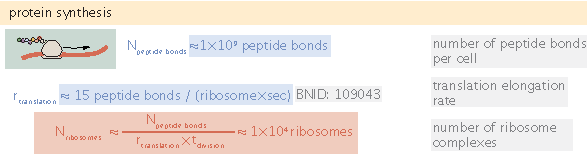
\includegraphics{main_figs/protein_synthesis.pdf}
        \caption{\textbf{Estimation of the required tRNA synthetases and
        ribosomes.} (A) Estimation for the
        number of tRNA synthetases that will supply the required amino acid
        demand. The sum of all tRNA synthetases copy numbers are plotted as a
        function of growth rate ([ArgS], [CysS], [GlnS], [GltX], [IleS], [LeuS],
        [ValS], [AlaS]$_2$, [AsnS]$_2$, [AspS]$_2$, [TyrS]$_2$, [TrpS]$_2$,
        [ThrS]$_2$, [SerS]$_2$, [ProS]$_2$, [PheS]$_2$[PheT]$_2$, [MetG]$_2$,
        [lysS]$_2$, [HisS]$_2$, [GlyS]$_2$[GlyQ]$_2$). (B) Estimation for the
        number of ribosomes required to synthesize all proteins in the cell. The
        average abundance of ribosomes is plotted as a function of growth rate.
        Our estimated values are shown for a growth rate of 0.5 hr$^{-1}$.}
    \label{fig:protein_synthesis}
    }
    \end{fullwidth}
\end{figure}

We can begin to gain some intuition into how translation might limit growth by
noting that the total number of peptide bonds generated as the cell doubles,
$N_{aa}$, which we used in our calculation above, will be given by, $\tau \cdot
r_t \cdot R$. Here, $\tau$ refers to the doubling time of the cell under
steady-state growth, $r_t$ is the maximum translation elongation rate, and $R$
is the average number of ribosomes per cell. With the growth rate related to the
cell doubling time by $\lambda = ln(2)/\tau$, we can write the
translation-limited growth rate as,

\begin{equation}
\lambda_{\textrm{translation-limited}} = \frac{ln(2) \cdot r_t \cdot R}{N_{aa}}.
\end{equation}
Alternatively, since $N_{aa}$ is related to the total protein mass through the
molecular weight of each protein, we can also consider the growth rate in terms
of ribosomal mass fraction. By making the approximation that an average amino
acid has a molecular weight of 110 Da (see \FIG{translation_1}(A)), we can
rewrite the growth rate as,

\begin{equation}
\lambda_{\textrm{translation-limited}} \approx \frac{ln(2) \cdot r_t}{L_R}  \Phi_R,
\label{eq:translation_limit_growth_rate}
\end{equation}
where $L_R$ is the total length in amino acids that make up a ribosome, and
$\Phi_R$ is the ribosomal mass fraction. This is plotted as a function of
ribosomal fraction $\Phi_R$ in \FIG{translation_1}(A), where we take $L_R
\approx $7459 aa, corresponding to the length in amino acids for all ribosomal
subunits of the 50S and 30S complex. This formulation assumes that the cell can
transcribe the required amount of rRNA, which appears reasonable for  \textit{E.
coli} under the  allowing us to consider the inherent limit on growth set by the
ribosome.

The growth rate defined by Equation \ref{eq:translation_limit_growth_rate}
reflects  mass-balance under steady-state growth and has long provided a
rationalization to the apparent linear increase in \textit{E. coli}'s ribosomal
content as a function of growth rate \citep{Goldberger1979, scott2010}. For our
purposes, there are several important consequences of this  trend. Perhaps the
first thing to notice is that there is a maximum growth rate at about $\lambda
\approx 6 hr^{-1}$, or doubling time of about 7 minutes (dashed line). This
growth rate can be viewed as an inherent maximum growth rate due to the need for
the cell to double the cell's entire ribosomal mass. Interestingly, this limit
is independent of the absolute number of ribosomes, but rather is simply given
by time to translate an entire ribosome, $L_R/ r_t$. As shown in
\FIG{translation_1}(B), we can reconcile this with the observation that in order
to double the average number of ribosomes, each ribosome must produce a second
ribosome. This is a process that cannot be parallelized.

For reasonable values of $\Phi_R$, between about 0.1 - 0.3 \citep{scott2010},
the maximum growth rate is in line with experimentally reported growth rates
around 0.5 - 2 $hr^{-1}$. Here we are implicitly assuming that translation
proceeds randomly, without preference between ribosomal or non-ribosomal mRNA,
which appears reasonable. Importantly, in order for a cell to scale this growth
limit set by $\Phi_R$, cells \textit{must} increase their ribosomal abundance.
This can be achieved by either synthesizing more ribosomes or reducing the
fraction of non-ribosomal proteins. Reduction of non-ribosomal proteins is not
straight forward since, as we have found throughout our estimates, doubling a
cell requires a substantial number of other enzymes and transporters. Increasing
the absolute ribosomal abundance is limited by the number of rRNA operons.

\begin{figure}
  \begin{fullwidth}
        \centering{
            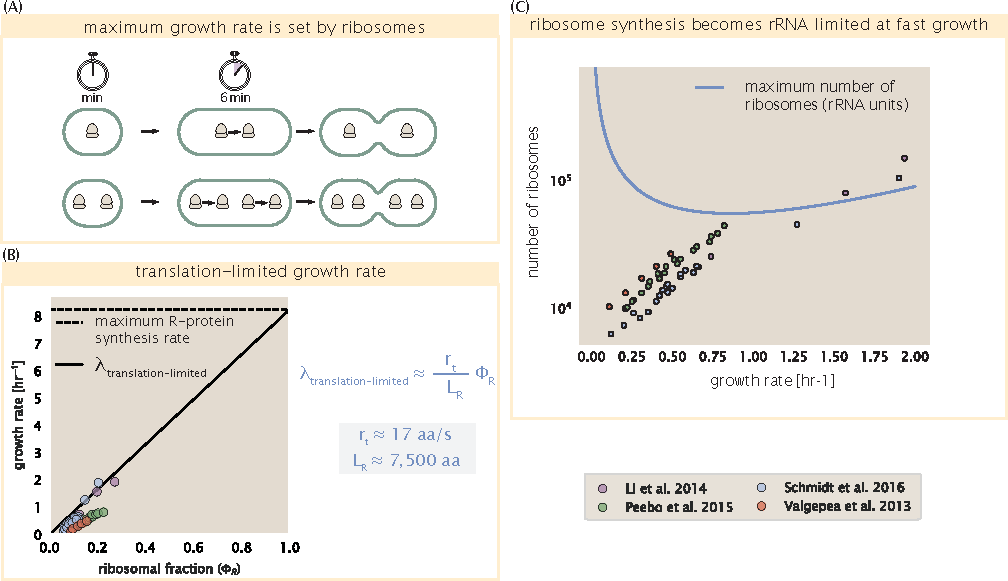
\includegraphics{main_figs/fig7_ribosome_growth_limit_2.pdf}
            \caption{\textbf{Translation-limited growth rate.} (A) Here we
            consider the translation-limited growth as a function of ribosomal
            fraction. By mass balance, the time required to double the entire
            proteome ($N_{aa}$ /$r_t \cdot $) sets the translation-limited
            growth rate, $\lambda_{\textrm{translation-limited}}$. Here $N_{aa}$
            is effectively the number of peptide bonds that must be translated,
            $r_t$ is the translation elongation rate, and $R$ is the number of
            ribosomes. This can also be re-written in terms of the ribosomal
            mass fraction $\Phi_R = m_R$ / $m_{\textrm{protein}}$, where $m_R$
            is the total ribosomal mass and $m_{\textrm{protein}}$ is the mass
            of all proteins in the cell. $L_R$ refers to the summed length of
            the ribosome in amino acids.
            $\lambda_{\textrm{translation-limited}}$ is ploted as a function of
            $\Phi_R$ (solid line). (B) The dashed line in part (A) identifies a
            maximum growth rate that is set by the ribosome. Specifically, this
            growth rate corresponds to the time required to  translation an
            entire ribosome, $L_R/ r_t$ . This is a result that is independent
            of the number of ribosomes in the cell as shown schematically here.
            (C) Schematic showing translation-specific requirements for maintenance
            of steady-state growth. In a nutrient rich environment, amino acid supply $r_{aa}$ is sufficiently in
            excess of demand by ribosomes translating at their maximal rate. In poorer
            nutrient conditions, reduced amino acid supply $r_{aa}$ will decrease
            the rate of elongation. In a regime where $r_{aa}$ is less than $r_t \cdot R$,
            the number of actively translating ribosomes will need to be reduced in order
            to maintain steady-state growth.}
        \label{fig:translation_1}
        }
  \end{fullwidth}
\end{figure}

While it is common for bacteria to decrease their ribosomal abundance in poorer
nutrient conditions \cite{scott2010, liebermeister2014}, this does not decrease
to zero. From the perspective of a bacterium dealing with uncertain nutrient
conditions, there is likely a benefit for the cell to maintain some relative
fraction of ribosomes to support rapid growth as nutrient conditions improve.
However, if we consider a scenario where nutrient conditions become poorer and
poorer, there will be a regime where ribosomes are in excess of the nutrient
supply. If the cell is to maintain steady-state growth, it will need to
attenuate its translational activity since ribosomes would otherwise exhaust
their supply of amino acids and bring cell growth to a halt
(\FIG{translation_1}(C)). In the next section we will consider this more
specifically for \textit{E. coli}, which has been shown to maintain a relatively
high elongation rate even in stationary phase ($\approx$ 8 aa/s, \cite{dai2016})
where cell growth is minimal.

[NB: I'm considering moving this paragraph near the end of the next section].

% In addition,
% given their massive size at about 850 kDa, they may play an as-yet fully
% understood role as a crowding agent in cellular function \cite{delarue2018,
% solerbistue2020}.

\subsection{Multiple replication forks bias ribosome abundance.}

\textit{E. coli} cells grow by an adder mechanism, whereby cells add a constant
volume with each cell division \citep{taheriaraghi2015}. In conjunction with
this, additional rounds of DNA replication are triggered when cells reach a
critical volume per origin of replication (\FIG{translation_ecoli}(A)). This
leads to the classically-described exponential increase in cell size with growth
rate \cite{schaechter1958, si2017, si2019}. In the context of maximizing growth
rate, it is notable that the majority of ribosomal proteins and rRNA operons are
found closer to the DNA origin. Given the need to increase to total gene dosage
of rRNA operons at faster growth rates, and the intimate relationship between ribosomal
content and growth rate we considered above, this raises the possibility that the
observed size scaling and increase in chromosomal content might simply be
a means for the cell to tune biosynthesis according to its
physiological state.

While an increase in transcription has been observed for genes near the origin
in rapidly growing \textit{E. coli}  \citep{scholz2019}, we were unaware of such
characterization at the proteomic level. In order to test whether there is a
relative increase in protein expression for genes closer to the origin, we
calculated a running boxcar average of protein copy number as a function of
each gene's transcriptional start site. While absolute protein copy numbers can vary
substantially across the chromosome, we indeed observe a bias in expression
under fast growth conditions (\FIG{translation_ecoli}(B), showing the result
using a 0.5 kb averaging window). The dramatic change in protein copy number
near the origin mainly reflects the increase in ribosomal protein expression.
This trend is in contrast to slower growth conditions where the average copy
number is more uniform across the length of the chromosome.

\begin{figure*}
    \begin{fullwidth}
    \centering{
        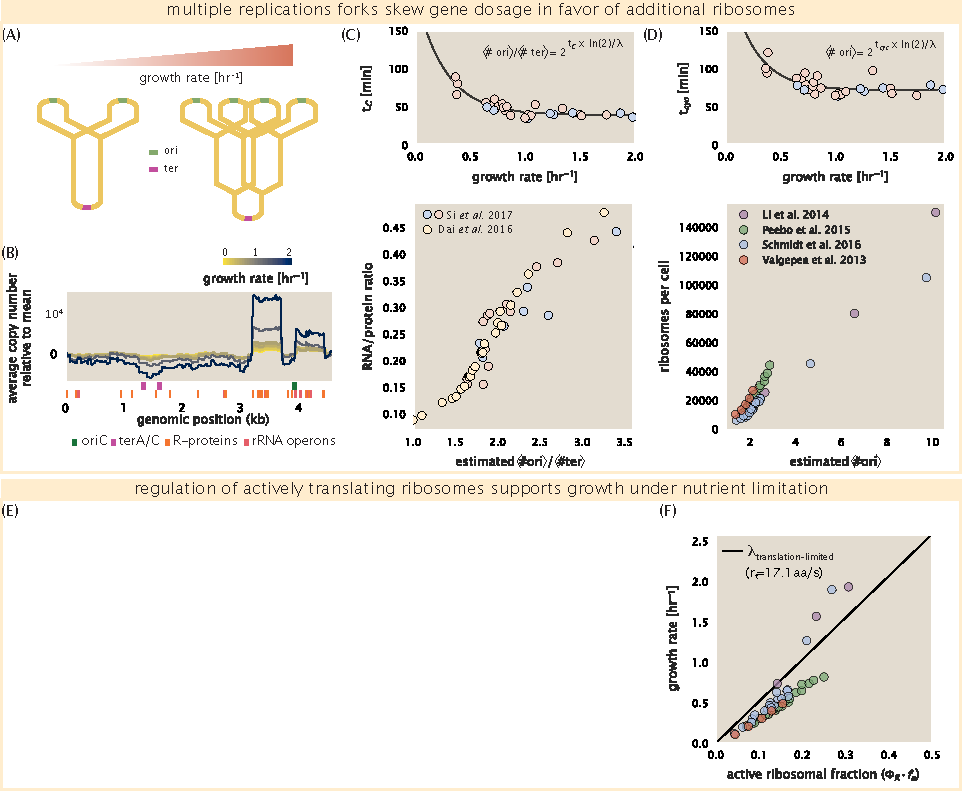
\includegraphics{main_figs/fig8_ribosome_growth_limit_ecoli_temp.pdf}
        \caption{\textbf{Multiple replication forks skew gene dosage and
        ribosomal content.} (A) Schematic shows the expected
        increase in replication forks (or number of ori regions) as \textit{E. coli} cells
        grow faster. (B) A running boxcar average of protein copy number is calculated for
        each each growth condition considered by
        Schmidt \textit{et al.}. A 0.5 kb averaging window was used. Protein
        copy numbers are reported relative to their condition-specific means in order to center all
        data sets.
        (C) and (E) show experimental data from Si \textit{et al.} (2017)
        Solid lines show fits to the data, which were used to estimate
        $\langle$\# ori$\rangle$ / $\langle$\# ter$\rangle$ and $\langle$\# ori$\rangle$
        [NB: to note fit equations]. Red data points correspond to measurements in strain
        MG1655, while light green points are for strain NCM3722. (D) Plot compares our estimate of
        $\langle$\# ori$\rangle$ / $\langle$\# ter$\rangle$  to the experimental
        measurements of ribosomal abundance. Ribosomal fraction was approximated from
        the RNA/protein ratios of Dai \textit{et al.} (2016) (yellow) and Si \textit{et al.} (2017) (light red and light green) by the conversion RNA/protein ratio $\approx \Phi_R \cdot 2.1$.
        (F) plots the ribosome copy number estimated from the proteomic data against
        our estimate of $\langle$\# ori$\rangle$.
        (G) [in progress], (H) Experimenta data from Dai \textit{et al.} are
        used to estimate the fraction of actively translating ribosomes. The
        solid line represents the translation-limited growth rate for ribosomes
        elongating at 17.1 aa/s. }
        \label{fig:translation_ecoli}
    }
    \end{fullwidth}
\end{figure*}

If ribosomal genes (rRNA and ribosomal proteins) are being synthesized according
to their available gene dosage we can make two related hypotheses about how
their abundance should vary with chromosomal content. The first is that the
ribosomal protein fraction should increase in proportion  to the average ratio of
DNA origins to DNA termini ($\langle$\# ori$\rangle$ / $\langle$\# ter$\rangle$
ratio). This is a consequence of the skew in DNA dosage as cells grow faster.
The second is that the absolute number of ribosomes should increase in proportion to the number of DNA origins ($\langle$\# ori$\rangle$), since this will reflect the total gene dosage at a particular growth condition.

In order to test eahc of these expectations we considered the experimental data
from Si \textit{et al.} (2017), which inferred these parameters for cells under
nutrient-limtied growth. $\langle$\# ori$\rangle$ / $\langle$\# ter$\rangle$
ratio) depends on how quickly chromosomes are replicated relative the cell's
doubling time $\tau$ and is given by 2$^{\tau_C / \tau}$. Here $\tau_C$ is the
time taken to replicate \textit{E. coli}'s' chromosome, referred to as the C
period of cell division.  In \FIG{translation_ecoli}(C) we plot $\tau_C$ versus
$\tau$ that were measured, with data points in red corresponding to \textit{E.
coli} strain MG1655, and blue to strain NCM3722. In their work they also
measured the total RNA to protein ratio  which reflects ribosomal abundance and
we show that data along with other recent  measurements from Dai \textit{et
al.}. Indeed we find that the ribosomal fraction increases with $\langle$\#
ori$\rangle$ / $\langle$\# ter$\rangle$ (\FIG{translation_ecoli}(C)). Across our
different proteomic data sets there also appeared two distinct trends. To
consider the possibility that this may reflect systematic differences in how the
data was generated, we also considered recent measurements of total RNA to
protein ratio across the growth rates considered, which provide an alternatic
measure of ribosomal abundance (RNA to protein ratio $\approx \Phi_R$ x 2.1
\cite{dai2016}). While these showed a similar correlation, they were most
consistent with the proteomic data from Schmidt \textit{et al.} (2016) and Li
\textit{et al.} (2014).

We can similarly estimate $\langle$\# ori$\rangle$, which depends on how often
replication forks are initiated per cell cycle. This is given by the number of
overlapping cell cycles,  2$^{\tau_{cyc} / \tau}$, where $\tau_{cyc}$, refers to
the total time of chromosome replication and cell division.
\FIG{translation_ecoli}(E) shows the associated data from Si \textit{et al.},
which we use to estimate $\langle$\# ori$\rangle$  for each growth condition of
the proteomic data. In agreement with our expectations, we find a strong
correlation between the ribosome copy number and estimated $\langle$\#
ori$\rangle$ (\FIG{translation_ecoli}(F)).

[NB: to do. 1) slow growth regime, 2) putting it all together ; cells appear to
grow near the translation-limited rate ($r_t$ = 17aa/s) across all growth coniditions. Need
to provide some rationalization for points above line. Maybe it's the interpretation
of $L_R$, or the reality that a ribosome complex is more complex than the simple picture of a 50S + 30S subunit consisdered here. In any case, in the fast growth regime, this amounts to
differences of ~minutes. ]

[NB: to incorporate. Titration of the cellular ppGpp concetration invoked similar proteomic changes
to those observed under nutrient limitation \citep{zhu2019}. In light of our
hypothesis that such changes to the proteome are intimately linked to  the
details of DNA replication, it was recently shown that both the  $\langle$\#
ori$\rangle$ / $\langle$\# ter$\rangle$ and cell size lost their growth rate
dependent scaling in a ppGpp null strain. Rather, cells exhibit a $\langle$\#
ori$\rangle$ / $\langle$\# ter$\rangle$ closer to 4 and cell size more
consistent with a fast growth state \citep{fernandezcoll2020}. This supports the
possibility that in addition  to coordinating ribosome activity, (p)ppGpp
signaling may be acting to coordinate other  cellular processes in accordance
with nutrient conditions and biosynthetic demand. From this  perspective, the
increase in the rate of DNA initation and associated increase in cell  size may
be viewed as a way for the cell to vary its proteomic composition and
biosynthetic  capacity according to its available nutrient conditions. ]


% ability to begin replication of multiple copies of its genome
% during a single cell cycle. This is achieved through multiple initiation forks
% and nested DNA replication. [need to refer to work from to Jun lab here!! -
% under adder mechanism, the cell appears to add a certain cell mass in proportion
% to its number of origins]. We find that the ribosome copy number increases in
% proportion to the expected number of origins. The process of nested DNA
% replication will lead to a bias in gene dosage for genes closer to the origin of
% replication \cite[], Importantly, ribosomal protein and rRNA genes are closer to
% the origin of replication \cite{scholz2019} and this provides a natural way for
% \textit{E. coli} to bias the proportion of ribosomes at faster growth without
% the advent of additional gene regulation strategies. Given that ribosomal genes
% in \textit{E. coli} appear to be transcribed at their maximal rate at fast
% growth rates [cite??],  increasing ribosomal copy number through increased gene
% dosage represents a creative  approach for the cell to grow faster without gross
% down-regulation of non-ribosomal genes.

% Next consider growth below the capacity of ribosomes.


% Maybe start with E. coli section by noting details from Jun lab as a given. Si et al 2017: The average cell size increased exponentially with respect to the nutrient-imposed growth rate l ( = ln2/t), in agreement with the nutrient growth law [1] (Figure 1; see the Supplemental Information). The ribosome fraction 4R increased linearly with the growth rate, confirming previous re- ports [8, 9]. tC and tcyc were both constant for a wide range of growth conditions at tC = 38.00 ± 4.50 and tcyc = 75.10 ± 7.20 (Fig- ure 1C; see the Supplemental Information) [21, 22].
%  AND it follows 'adder' model of cell division

%  Noting Fig7A, highlight that for cells to optimize their growth , they will benefit by varying their ribosomal abundance; and that they can do this by varying gene dosage - since otherwise it is not obvious how they might make more ribsoomes.

% ****** Data from that 2020 paper on ppGpp and Si et al, and Zhu et al. all point to an increase in ribosomal content with higher number of origins (t_cyc/ tau)
% ->> Can I show this somehow , maybe an important point.



% Might be worth noting that E. coli doesn't grow if you knockout regulation by ppGpp. FROM Zhu et al. 2019 NAR: On the other hand, low ppGpp levels seem to be adverse for biomass growth as well, as shown by the inability of ppGpp- null strain to grow in minimal medium (21,32,33), suggest- ing the importance of maintain an optimal ppGpp level for cell growth.

% It'll remain to be determined whether perturbations like those in Dai et al.,
% and the more recent paper in NAR is consistent with a varying number of
% origins. But I think it's curious that they see a trend exactly like the trend
% in nutrient-limited growth when they vary ppGpp, and roughly similar (high)
% active fraction of ribosomes. I guess is that this type of regulation works
% on more than just ribosomes, and perhaps it is changing number of origins.
% Another point is that fraction of ribosomes again seems to move toward
% a non-zero limit, which bodes well with number of ribosomes depending on
% number of DNA ori.

% I don't think it's trivial to 'up' regulate ribosomal synthensis. This seems like an importsnt consideration.

% I think it might be worth noting that we can think of this changing gene dosage as also changing the genome makeup of the cell.

\subsection{Maximum Growth Rate is Determined by the Ribosomal Mass Fraction}
We begin by considering the length of time needed to replicate a single
ribosome. As mentioned in our discussion of rRNA synthesis, the bacterial
ribosome is approximately 2/3 RNA by mass, with the remaining 1/3 being composed
of protein. Of the $\approx$ 50 ribosomal subunits, all are present as a single
copy save for RplL which is present in four copies. Taking these proteins
together, a single ribosome is composed of $L_R \approx$ 7500 individual amino
acids, approximately equal to the number of peptide bonds. Again assuming a
reasonable translation rate of $r_t \approx$ 15 amino acids per second, we arrive at
an simple estimate that it takes on the order of  $L_R / r_t \approx$ 7 minutes to
translate a single ribosome. This limit, as remarked upon by others
\citep{dill2011}, serves as a hard limit for how quickly \textit{E. coli} could
replicate. As each ribosome would therefore need to copy itself, this  7 minute
speed limit is independent of the number of ribosomes per cell
(\FIG{ribosome_limit}(A)), yet assumes that the only proteins that need
to be replicated for division to occur are ribosomal proteins, a regime we know is not met in
biological reality. 

However, we can consider the translation limited growth rate as a function of
the fraction $\Phi_R$ of the total number of amino acids in the proteome $N_\text{pep}$
that are sequestered in a ribosome, $N_\text{pep}^\text{(ribosome)}$. To compute this quantity, we
note that the number of amino acids in a ribosome is related to the protein mass
via 
\begin{equation}
  m_\text{ribosome} \approx L_R \times m_\text{AA}
  \label{eq:mribo}
\end{equation}
where $m_\text{AA}$ is the average mass of an amino acid which is $\approx$ 110
Da (BNID: 104877). Similarly, we can compute the mass of the total cellular
proteome as 
\begin{equation}
  m_\text{proteome} \approx N_\text{pep} \teims m_\text{AA}.
  \label{eq:mproteome}
\end{equation}

Together, \EQ{mribo} and \EQ{mproteome} allow us to define the ribosomal mass
fraction as 
\begin{equation}
  \Phi_R = \frac{m_\text{ribosome} \times R}{m_\text{proteome}} \approx \frac{R \times L_R}{N_\text{pep}}.
  \label{eq:phir}
\end{equation}
Relating the number of peptide bonds to be synthesized to complete division to
the number of ribosomes per cell in this manner allows us to enumerate an
expression for translation-limited growth. As cells grow exponentially in time
\cite{godin2010}, the rate of cellular growth can be computed as 
\begin{equation}
N_\text{pep} \lambda = r_t \times R \times f_a,
\label{eq:exp_cell_growth}
\end{equation}
where $\lambda$ is the cellular growth rate and $f_a$ is a multiplicative factor
which describes the fraction of ribosomes actively translating. This latter term
allows us to account for the possibility of nonfunctional, immature ribosomes or
active sequestration of ribosomes through small-molecule alarmones such as
(p)ppGpp which can be significant at slow growth rates \citep{dennis2004,
dai2016}. Combining \EQ{phir} and \EQ{exp_cell_growth} yields an expression for
the translation limited growth rate 
\begin{equation}
\lambda_\text{translation-limited} \approx \frac{r_t}{L_R}\Phi_Rf_a.
\label{eq:lam_lim}
\end{equation}

This expression is plotted in the top panel of \FIG{limit}(B) assuming $f_a =
1$. When $\Phi_R \approx 1$ (i.e. when all proteins in the cell are ribosomal),
the maximum growth rate corresponds to the speed limit of $\approx$ 7 min,
illustrated by a dashed line in the top panel of \FIG{limit}(B). As the product
$f_a \times \Phi_R$ is
decreased, meaning the ribosomes occupy a smaller and smaller proportion of the
proteome, we observe that the growth similarly decreases. To make a connection
with the proteomic data, we require a means to estimate $f_a$ at each growth
rate. Recent measurements by \cite{dai2016} reveal that $f_a \approx 1$ at fast
growth rates ($>$ 0.75 hr$^{-1}$) and monotonically decreases as slower growth
rates (\FIG{limit} (B), inset in bottom plot). Using these data, we estimated
$f_a$ for each growth rate present in the proteomic data set. In general, these
data appear to skirt this translation limited growth regime as growth conditions
change (\FIG{limit}(B), colored points in bottom plot). There is a notable
discrepancy between the data collected in \cite{schmidt2016, li2014} and that
collected from \cite{valgepea2013, peebo2015}. When compared to other,
non-proteomic wide measurements of the active ribosome mass fraction
(\FIG{limit} (B), grey points in bottom plot), the data from \cite{valgepea2013}
and \cite{peebo2015} are notably aberrant, suggesting a systematic error in
these data. 


The translation-limited view of growth defined \EQ{lam_lim} reflects
mass-balance under steady state growth and has long provided a rationalization
of the apparent linear increase in \textit{E. coli}'s ribosomal content as a
function growth rate \cite{goldberger1979,schaechter1958,scott2010}. While this
is a useful framework to approximately consider how the relative abundance of ribosomes
(compared to all other proteins) defines the growth rate, it is worth noting
that as growth rate increases, so does the cell size and therefore so must the
proteome mass. With a handle on how elongation rate and the total number of
peptide bonds per proteome is related to the growth rate, we now expand this
description to account for the changing cell size, allowing us to consider a
potential bottleneck in the synthesis of rRNA.

% To  gain some intuition into how ribosomal synthesis influences
% bacterial growth, we again consider the total number of peptide bonds that must
% be synthesized, which we denote as $N_\text{pep}$. With cells growing exponentially in time
% \citep{godin2010}, the rate of cellular growth will be related to the rate of protein synthesis by
% \begin{equation}
%     N_\text{pep} \lambda = r_t R f_a,
%     \label{eq:mass_balance}
% \end{equation}
% where $\lambda$ is the cell growth rate,  $r_t$ is the maximum
% elongation rate in AA per second, and $R$ is the average ribosome copy
% number per cell. The multiplicative factor $f_a$ refers to the fraction of
% ribosomes actively translating, and allows us to account for the possibility of
% nonfunctional, immature ribosomes or active sequestration of ribosomes, mediated
% by the secondary-messenger molecule alarmones, such as guanosine pentaphosphate
% [(p)ppGpp] at slow growth \citep{dennis2004, dai2016}.

% Rather than speaking in terms of absolute ribosome abundance, we can account for
% the ribosome content as was defined by \cite{scott2010} as the mass of fraction
% of the proteome occupied by ribosomes $\Phi_R$. Similarly, as $N_\text{pep}$ is related to
% the total protein mass through the molecular weight of each protein, we can also consider the growth
% rate in terms of the fraction of the total proteome mass dedicated to ribosomal
% proteins. By making the approximation that an average amino acid has a molecular
% weight of 110 Da (BNID: 104877), the total protein mass $m_\text{protein}$ is
% related to $N_\text{pep}$ by $(m_\text{protein}/\text{110 Da}) \times N_A$,
% where $N_A$ is Avogadro's number. Similarly, $R$ is related to the ribosomal
% protein mass by $R \approx (m_R/\text{800 Da}) \times N_A$, where 800 Da
% reflects the summed molecular weight of all ribosomal subunits.  This allows us
% to approximate  $R / N_\text{pep} \approx \Phi_R / L_R$,  where $\Phi_R$ is the
% ribosomal mass fraction $m_\text{protein}/m_R$, and $L_R$ the ratio of 800 kDa /
% 110 Da per amino acid or, alternatively, the total length in amino acids that
% make up a ribosome. Under this parameterization, the translation-limited growth rate can then be written in
% the form
% \begin{equation}
% \lambda_{\textrm{translation-limited}} \approx \frac{r_t}{L_R}  \Phi_R f_a.
% \label{eq:translation_limit_growth_rate}
% \end{equation}
% This is plotted as a function of the ribosomal fraction $\Phi_R$ in the top panel of
% \FIG{ribosome_limit}(A), where we take $L_R \approx$ 7500 AA, corresponding to
% the length in amino acids for all ribosomal subunits of the 50S and 30S complex
% (BNID: 101175), and $f_a$ = 1. To compare this relationship to the proteomic
% data, we make use of recent measurements of $f_a$ from \cite{dai2016}
% (\FIG{ribosome_limit}(A), bottom inset) to estimate the active
% fraction of ribosomal protein across each proteomic data set
% (\FIG{ribosome_limit}(A), colored points, bottom). In general, the data appear to
% skirt this limit in growth rate as nutrient conditions vary. There is a notable discrepancy
% in the data from \cite{peebo2015, valgepea2013}, where cells appear to grow
% substantially slower given their estimated ribosomal fraction. Here we have
% also collected a number of recent non-proteomic measurements of ribosomal fraction and
% find them most consistent with the measurements from \cite{li2014,
% schmidt2016} (gray points; also see \FIGSUPP[ribosome_limit]{ribosome_limit_supp}(A)).

% The growth rate defined by \EQ{translation_limit_growth_rate} reflects
% mass-balance under steady state growth and has long provided a rationalization
% of the apparent linear increase in \textit{E. coli}'s ribosomal content as a
% function of growth rate \citep{goldberger1979, scott2010}. The maximum rate,
% when $\Phi_R$ = 1, could only be achieved if a cell contained only ribosomes \citep{dill2011}.
% This corresponds to the synthesis time of all ribosomal subunits, $L_R/ r_t
% \approx$ 7 minutes and interestingly, is independent of the
% absolute number of ribosomes (\FIG{ribosome_limit}(B)). To return to our earlier comments on
% parallelization, it is this step that is rate-limiting, with each ribosome being
% required to produce a second ribosome. Unless elongation rate increased, or
% cells could trim their total ribosomal protein mass, this dependency limits both
% the maximum growth rate (when $\Phi_R$ = 1), and also the achieveable growth
% rate under more moderate values of $\Phi_R$.

\begin{figure}
  \begin{fullwidth}
        \centering{
        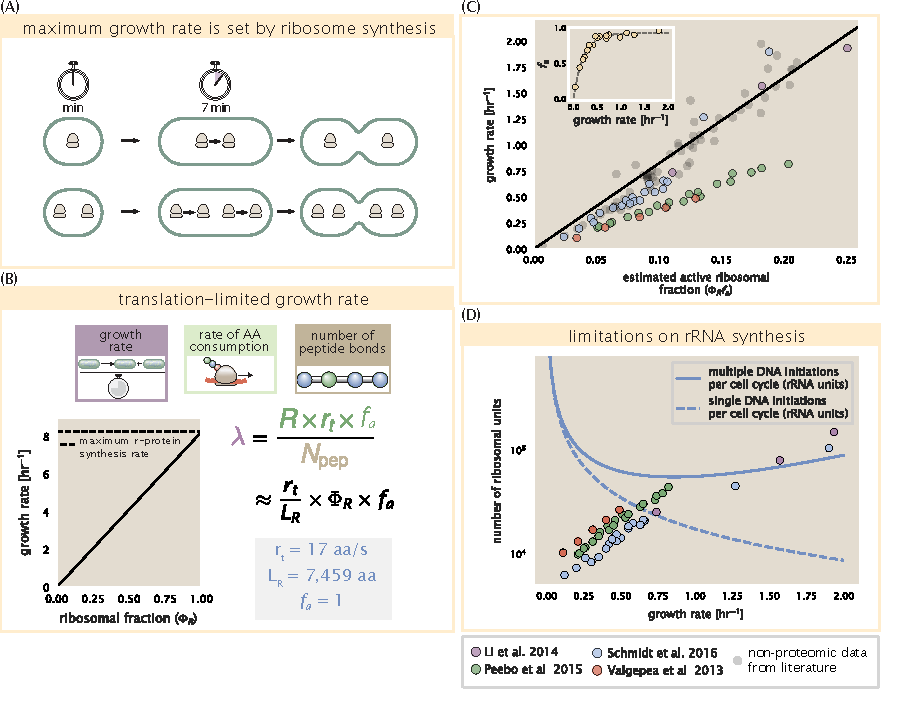
\includegraphics{main_figs/fig7_ribosome_as_limit.pdf}
        \caption{\textbf{Translation-limited growth rate.}  (A) \textit{top}:
        Translation-limited growth as a function of the ribosomal fraction. The
        solid line is calculated for an elongation rate of 17 aa per second.
        The dashed line corresponds to the maximum rate of ribosomal protein
        (R-protein) synthesis considered in part (C).
        \textit{bottom}: Actively translating ribosomal fraction versus growth rate.
        The actively translating ribosomal fraction is calculated using the
        estimated values of $f_a$ from  \cite{dai2016} (shown in inset; see
        Appendix \nameref{sec:SI_f_a} for additional detail). Gray data points
        show additional measurements from literature and consider further in
        \FIGSUPP[ribosome_limit]{ribosome_limit_supp}(A).
        (B) An inherent
        maximum growth rate is set by the time to synthesize all ribosomal
        subunits. This growth rate is given by $r_t/ L_R$, where $r_t$ is
        the elongation rate and $L_R$ is the total number of amino acids
        that make up the entire ribosomal complex. This rate is independent
        of the number of ribosomes and instead is limited by the time required to
        double an individual ribosome.
        (C) Maximum number of
        rRNA units that can be synthesized as a function of growth rate.
        Solid curve corresponding to the rRNA copy number is calculated by
        multipyling the number of rRNA operons by the estimated number of
        $\langle\text{\# ori}\rangle$ at each growth rate. The quantity
        $\langle\text{\# ori}\rangle$ was calculated using Equation 4 and
        the measurements from \cite{si2017} that are plotted in
        \FIG{translation_ecoli_partA}(A). The dashed line shows the maximal
        number of functional rRNA units produced from a single chromosomal
        initiation per cell cycle. }
        \label{fig:ribosome_limit}


        \figsupp[Comparison of $\Phi_R f_a$ with literature and estimation of $\langle$\# ori$\rangle$.]{(A) Actively translating ribosomal fraction versus growth rate.
        The actively translating ribosomal fraction is calculated using the
        estimated values of $f_a$ from  \cite{dai2016} (shown in inset; see
        Appendix \nameref{sec:SI_f_a} for additional detail). Additional measurements
        in addition to the proteomic measurements are based on measurements of cellular RNA to
        protein ratio, with $\Phi_R \approx$ the cellular RNA to
        protein ratio divided by 2.1 \citep{dai2016}. (B) Experimental measurements of
        the cell doubling time $\tau$ and cell cycle time $t_{cyc}$
         from Si \textit{et al.}
        (2017). Dashed line shows fit to the data, which were used to estimate
        $\langle$\# ori$\rangle$. $t_{cyc}$ was assumed to vary in proportion to
        $\tau$ for doubling times greater than 40 minutes, and reach a
        minimum value of 73 minutes. See Appendix
        \nameref{sec:SI_ori} for additional details exact estimation of rRNA copy number. Red data points correspond
        to measurements in strain MG1655, while light green points are for
        strain NCM3722.
        Schematic shows the expected increase in replication forks (or number of
        ori regions) as \textit{E. coli} cells grow faster. }{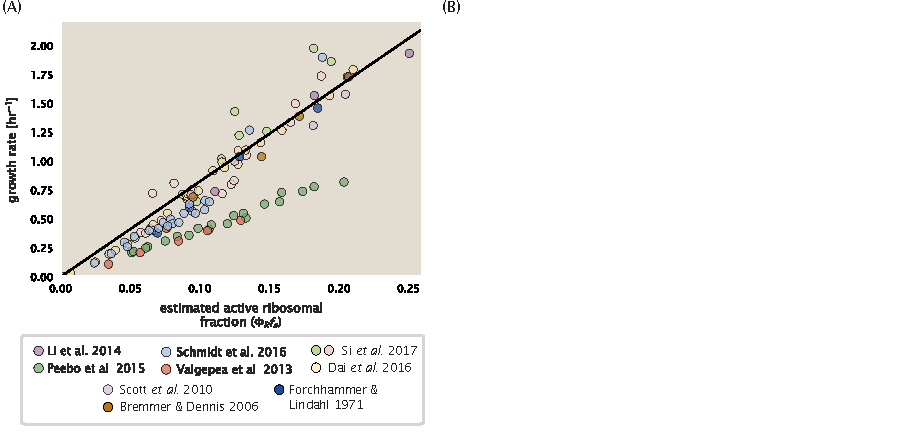
\includegraphics{main_figs/fig7_ribosome_as_limit_Supp.pdf}}\label{figsupp:ribosome_limit_supp}
        }
  \end{fullwidth}
\end{figure}

\subsection{rRNA Synthesis Presents a Potential Bottleneck during Rapid Growth}
\textit{E. coli} rarely exhibits growth rates above 2 hr$^{-1}$
\citep{bremer2008}, which is still well-below the synthesis rate of a single
ribosome, and below the growth rates reported for several other bacteria
\citep{roller2016}. Here we need to also consider ribosomal synthesis from the
perspective of limiting rRNA synthesis, which as we have found earlier, will depend on the
number of rRNA operons to transcribe rRNA.

Due to multiple rounds of chromosomal replication per cell doubling, the
effective number of rRNA operons increases with growth rate and will vary in
proportion to the average number of origins per cell, $\langle$\# ori$\rangle$.
This parameter is set by how often replication must be initiated per cell
doubling in order to maintain steady state growth, and quantified by
\begin{equation}
    \langle \text{\# ori} \rangle = 2^{\tau_{cyc} / \tau} = 2^{\tau_{cyc} \lambda / ln(2)}.
    \label{eq:Nori}
\end{equation}
Here, $t_{cyc}$ is the cell cycle time (referring to the time from replication
initiation to cell division), and $\tau$ is the cell doubling time.  We used the
experimental measurements of $\tau_{cyc}$ and  $\tau$ from \cite{si2017}
(\FIGSUPP[ribosome_limit]{ribosome_limit_supp}(B)) to calculate $\langle$\#
ori$\rangle$  with \EQ{Nori} as a function of growth rates. For growth rates
above about 0.5 hr$^{-1}$, $t_{cyc}$ is approximately constant at about 70
minutes, which means that $\langle$\# ori$\rangle$ will grow exponentially with
growth rate. Since the rRNA operons are predominantly located near to origin of
replication  (BNID: 100352, \cite{dennis2004}), we make the simplifying
assumption that that the number of rRNA operons  will be directly proportional
to $\langle$\# ori$\rangle$.

Returning to our rule-of-thumb of 1 functional rRNA unit per second per operon,
we estimate the maximum number of ribosomes that could be made as a function of
growth rate (\FIG{ribosome_limit}(C), blue curve). Although we expect this
estimate to drastically overestimate rRNA abundance at slower growth rates
($\lambda < 0.5\, \text{hr}^{-1}$), it provides a useful reference alongside the
proteomic measurements. For growth rates above about 1 hr$^{-1}$, we find that
cells will \textit{need} to transcribe rRNA near their maximal rate. As a counter
example, if \textit{E. coli} did not initiate multiple rounds of replication,
they would be unable to make enough rRNA for the observed number of ribosomes
(dashed blue curve in \FIG{ribosome_limit}(C)). The convergence between the
maximum rRNA production and measured ribosome copy number suggests rRNA
synthesis may begin to present a bottleneck at the fastest growth rates due to
the still-limited copies of rRNA genes.


% It is now well-documented that \textit{E. coli} cells add a constant volume per
% origin of replication, which is robust to a remarkable array of cellular
% perturbations \citep{si2017}.

% To consider
% this  in the context of the proteomic data, we used measurements of $\tau_{cyc}$
% and  $\tau$ from \cite{si2017} (\FIG{translation_ecoli_partA}(A)) to
% calculate $\langle$\# ori$\rangle$  with \EQ{Nori} at different growth
% rates. For ribosomal synthesis, we find an approximately linear correlation
% between ribosome copy number and $\langle$\# ori$\rangle$
% (\FIG{translation_ecoli_partA}(B)).
%
% For a constant cell cycle time, which is observed at growth rates above about
% 0.5 hr$^{-1}$ (\FIG{translation_ecoli_partA}(A), \citep{helmstetter1968}),
% \EQ{Nori} states that $\langle \text{\# ori} \rangle$ will need to increase
% exponentially with the growth rate.

% \subsection{Rapid Growth Requires \textit{E. coli} to Increase Both Cell Size and Ribosomal
Mass Fraction}
In the right-hand side of \FIG{ribosome_limit}(B),  we also find that above about 0.75
hr$^{-1}$, the growth rate is determined solely by the ribosomal mass fraction
$\Phi_R$, since $f_a$ is close to 1, and $r_t$ is near its maximal rate
\citep{dai2016}. While $\Phi_R$ will need to increase in order for cells to
grow faster, the fractional dependence in \EQ{lam_limited}
gives little insight into how this scaling is actually achieved by the cell.

It is now well-documented that \textit{E. coli} cells add a constant volume per
origin of replication, which is robust to a remarkable array of cellular
perturbations \citep{si2017}. Given the proteomic measurements featured in this
work, we find that the ribosome copy number also scales in proportion to
$\langle$\# ori$\rangle$ (\FIG{translation_ecoli_partA}(A)). However,  an
increase in ribosome abundance alone is not necessarily sufficient to increase
growth rate and  we also need to consider how $\Phi_R$ varies with $\langle$\#
ori$\rangle$. Importantly, as shown in \FIG{translation_ecoli_partA}(B), we find
that the deviations in protein expression with $\langle$\# ori$\rangle$ are
largely restricted to regions of ribosomal protein genes
\FIG{translation_ecoli_partA}(B). Here we have calculated the position-dependent
protein expression across the chromosome by a running Gaussian average of
protein copy number (20 kbp st. dev. averaging window) based on each gene's
transcriptional start site. These were median-subtracted to account for the
change in total protein abundance with $\langle$\# ori$\rangle$. This result
suggests that $\Phi_R$ is also being tuned in proportion to $\langle$\#
ori$\rangle$ under nutrient-limited growth, and in particular, it is through
this additional dependence on $\Phi_R$, combined with the exponential increase
in $\langle$\# ori$\rangle$, that \textit{E. coli} exhibits an exponential
increase in cell size with growth rate.

% To understand how this relates to growth rate, we
% neeed to consider the changes in proteome composition and ribosome abundance
% with $\langle$\# ori$\rangle$. In \FIG{translation_ecoli_partA}(D),


% For a
% constant cell cycle time $\tau_{cyc}$, which is observed at growth rates above
% about 0.5 hr$^{-1}$ (\FIG{translation_ecoli_partA}(A), \citep{helmstetter1968}),
% \EQ{Nori} states that $\langle \text{\# ori} \rangle$ will need to increase
% exponentially with the growth rate.

%
%
%
% While this says nothing of the observed scaling between cell
% size and growth rate, the additional dependency on ribosomal fraction through
% \EQ{translation_limit_growth_rate} provides an important link.
%
%



%
% To better explore how cells vary protein abundance proteome-wide
% across growth conditions, in \FIG{translation_ecoli_partA}(D), we show that the major deviations
% in protein expression across the chromosome in different growth conditions is a change
% in ribosomal expression.
%
% determined the position-dependent protein expression across the chromosome by
% calculating a running Gaussian average of protein copy number (20 kbp st. dev.
% averaging window) based on each gene's transcriptional start site. These were
% median-subtracted to account for the differences in total protein abundance.
%

%
%
% \subsection{Rapid Growth Requires an Increase in Ribosomal Copy Number and Cell Size}
% In \FIG{ribosome_limit}(C) we find that above about 0.75 hr$^{-1}$, the growth
% rate is dictated by the ribosomal mass fraction $\Phi_R$, since $f_a$ is close
% to 1, and $r_t$ is near its maximal rate [cite and refer to figure/
% supplemental]. While the preceeding section helps us understand that cells will
% need to increase $\Phi_R$ in order to grow faster, the fractional dependence
% gives little insight into how this is actually achieved within the cell. Here we
% consider how the observed changes in absolute protein content
% relate to this dependence between growth rate and $\Phi_R$.
%
% It is now well-documented that \textit{E. coli} cells add a constant volume per
% origin of replication, which is robust to a remarkable array of cellular
% perturbations \citep{si2017}.  The average number of origins per cell, $\langle$\#
% ori$\rangle$, is set by how often replication must be initiated per cell doubling
% under steady state growth. This can be quantified as
% \begin{equation}
%     \langle \text{\# ori} \rangle = 2^{\tau_{cyc} / \tau} = 2^{\tau_{cyc} \lambda / ln(2)},
%     \label{eq:Nori}
% \end{equation}
% where $t_{cyc}$ is the cell cycle time (referring to the time from replication
% initiation to cell division), and $\tau$ is the cell doubling time. To consider
% this  in the context of the proteomic data, we used measurements of $\tau_{cyc}$
% and  $\tau$ from \cite{si2017} (\FIG{translation_ecoli_partA}(A)) to
% calculate $\langle$\# ori$\rangle$  with \EQ{Nori} at different growth
% rates. For ribosomal synthesis, we find an approximately linear correlation
% between ribosome copy number and $\langle$\# ori$\rangle$
% (\FIG{translation_ecoli_partA}(B)).
%
% For a constant cell cycle time, which is observed at growth rates above about
% 0.5 hr$^{-1}$ (\FIG{translation_ecoli_partA}(A), \citep{helmstetter1968}),
% \EQ{Nori} states that $\langle \text{\# ori} \rangle$ will need to increase
% exponentially with the growth rate. While this says nothing of the observed
% scaling between cell size and growth rate, the additional dependency on
% ribosomal fraction through \EQ{translation_limit_growth_rate} provides an
% important link. To better explore how cells vary protein abundance proteome-wide
% across growth conditions, in \FIG{translation_ecoli_partA}(D), we
% determined the position-dependent protein expression across the chromosome by
% calculating a running Gaussian average of protein copy number (20 kbp st. dev.
% averaging window) based on each gene's transcriptional start site. These were
% median-subtracted to account for the differences in total protein abundance.
% Importantly, the major deviations in protein copy number are largely restricted to
% regions of ribosomal protein genes. This suggests that the ribosomal fraction
% $\Phi_R$ is also being tuned in proportion to $\langle$\# ori$\rangle$, and that
% it is through this dependence that \textit{E. coli} exhibits an exponential
% increase in cell volume with growth rate.




\begin{figure*}
    \begin{fullwidth}
    \centering{
        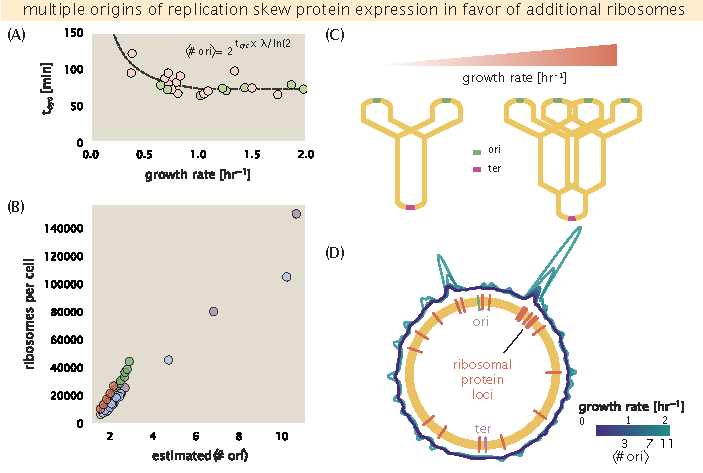
\includegraphics{main_figs/fig8_ribosome_growth_limit_ecoli_a_polar_coord.pdf}
        \caption{\textbf{Cells increase both absolute ribosome abundance and $\Phi_R$ with
        $\langle$\# ori$\rangle$.} (A) Plot of the ribosome copy number estimated from the
        proteomic data against the estimated $\langle$\# ori$\rangle$ (see Appendix
        \nameref{sec:SI_ori} for additional details). (B) A running
        Gaussian average (20 kbp st. dev.) of protein copy number is calculated
        for each growth condition considered by \citep{schmidt2016} based
        on each gene's transcriptional start site. Since total
        protein abundance increases with growth rate, protein copy numbers are
        median-subtracted to allow comparison between growth conditions.
        $\langle$\# ori$\rangle$ are estimated using the data in (A) and
        Equation \ref{eq:Nori}. } \label{fig:translation_ecoli_partA}
    }
    \end{fullwidth}
\end{figure*}


\subsection{Alarmone-Mediated Regulation Controls the Rate of Protein Synthesis}

As we have seen, cell size, total proteomic content, and the number of ribosomes
are all interconnected and influence the achievable growth rate. The drastic
change in these parameters across different growth conditions suggests that
they are being tuned to better match the cell's biosynthetic capacity to the
specific environment. Take, as another illustration of this, the recent
experimental work by \cite{dai2016}. In one set of experiments the authors
considered growth in cells whose primary glucose transport system was disrupted
($\Delta$\textit{ptsG}). Unsurprisingly, the growth rate was reduced, and was
measured at about two-fold slower than their wild-type line.  This change,
however, was not simply the result of now-limiting carbon uptake. Instead, cells
accomodated the perturbation by also reducing their ribosomal mass fraction by
a factor of two, which is still in line with \EQ{translation_limit_growth_rate}
under translation-limited growth.  In this final, we explore the interconnection
between cell size, ribosome content, and growth rate by formulating a minimal
model of growth rate control. We use it to quantitatively show how tuning these
parameters help cells maximize their growth rate.

To react to changes in nutrient conditions, bacteria rely on the synthesis or
degradation of secondary-messenger molecules  like (p)ppGpp, which cause global
changes in transcriptional and translational activity. In \textit{E. coli},
amino acid starvation causes the accumulation of de-acylated tRNAs at the
ribosome's A-site and leads to a strong increase in (p)ppGpp synthesis activity
by the enzyme RelA \citep{hauryliuk2015}. Cells also accumulate (p)ppGpp  during
steady-state growth in poorer growth conditions, which leads to a decrease in
the fraction of actively translating ribosomes, $f_a$  (with $f_a \approx 0.5$
at a growth rate of $\approx$ 0.3 hr$^{-1}$; \FIG{ribosome_limit}(C) - inset).

Furthermore, (p)ppGpp can inhibit the initiation of DNA replication by mediating
a change in transcriptional activity and the supercoiling state of the origin of
replication \citep{kraemer2019}. These observations all raise the possibility
that it is through (p)ppGpp that cells mediate the growth-rate dependent changes
in $\langle$\# ori$\rangle$, cell size, and ribosomal abundance and activity
\citep{zhu2019, Buke2020}. Indeed, recent work in a (p)ppGpp deficient strain of
\textit{E. coli} found that cells exhibited a high ratio of $\langle$\#
ori$\rangle$ to $\langle$\# ter$\rangle$, and cell sizes that were more
consistent with a fast growth state where (p)ppGpp levels are normally low
\citep{fernandezcoll2020}.

\subsection{Ribosomal Elongation Rate and Cellular Growth Rate are Linked by
Amino Acid Scarcity}
Here we consider a mode of regulation in which the rate of peptide elongation
$r_t$ depends only on the availability of amino acids (and, therefore, also
amino-acyl tRNAs). It is through the elongation rate $r_t$ that we assume cells
adjust their ribosomal content ($R$, $\Phi_R$) according to nutrient
availability and for simplicity, do not explicitly model changes in  $\langle$\#
ori$\rangle$ or regulation by (p)ppGpp.

The rate of elongation $r_t$ will depend on how quickly the ribosomes can match
codons with their correct amino-acyl tRNA, along with the subsequent steps of
peptide bond formation and translocation. We therefore coarse-grain the steps of
elongation to two time-scales,  1) the time required to find and bind each
correct amino-acyl tRNA, and 2) the remaining steps in peptide elongation that
will not depend on the amino acid availability. Under this model, other
molecular players required for translation like elongation factors and GTP are
considered in sufficient abundance, which appear to be valid assumptions given
our analysis of the proteomic data and energy production thus far. The time to
translate each codon is given by the inverse of the elongation rate $r_t$, which
can be written as,

\begin{equation}
\frac{1}{r_t} = \frac{1}{k_{on} \alpha [AA]_{\text{eff}}} + \frac{1}{r_{t}^{\text{max}}}.
\end{equation}
where we have assumed that the rate of binding by amino-acyl tRNA $k_{on}$ is
proportional to $[AA]_{\text{eff}}$ by a constant $\alpha$. The second term on
the right-hand side reflects our assumption that other steps in peptide
elongation are not rate-limiting, with a maximum elongation rate
$r_{t}^{\text{max}}$ of about 17 amino acids per second \cite{dai2016}. As the
rate of amino acid supply, denote by $r_{AA}$, varies with changing nutrient
condtions, the cell can maximize the rate of protein synthesis by tuning the
rate of amino acid consumption (mathematized as $r_t \times R \times f_a$) ,
shown schematically in \FIG{elongation_rate_model}(A). This can be stated more
succinctly in terms of an effective dissociation constant, $K_D = r_{t}^{\text{max}} / \alpha k_\text{on}$, where the elongation rate $r_t$ is now given by

\begin{equation}
r_t = \frac{r_{t}^{\text{max}}}{1 + K_D/[AA]_{\text{eff}}}.
\label{eq:rt_kd_simple}
\end{equation}

Under steady-state growth, the amino acid concentration is constant
($\frac{d[AA]_\text{eff}}{dt}=0$) and will relate to the rate of amino acid
synthesis (or import, for rich media) and/or tRNA charging, as $r_{AA}$, and the
rate of consumption, $r_t\times R \times f_a$ by,

\begin{equation}
\int_{0}^{t} \frac{d[AA]_{\text{eff}}}{dt} dt =  \int_{0}^{t}([r_{AA}] - [r_t\times R \times f_a]) dt,
\label{eq:aaeff_int}
\end{equation}
where the time from 0 to $t$ is an arbitrary length of time, and the square
brackets indicate concentrations per unit time. Integrating \EQ{aaeff_int}
yields,

\begin{equation}
   [AA]_\text{eff} = \frac{t(r_{AA} - r_t \times R \times f_a)}{V},
   \label{eq:aa_final}
\end{equation}
with  $r_{AA}$ is in units of AA per unit time and $r_t$ is in units of AA per
unit time per ribosome, for a cell with average volume $V$. Plugging \EQ{aa_final}
into \EQ{rt_kd_simple} allows us to then solve for $r_t$ and
a complete derivation is provided in Appendix \ref{sec:SI_model}.

In \FIG{elongation_rate_model}(B), we illustrate how the elongation rate depends
on the ribosomal copy number. Here, we have considered a unit volume $V =
1$\textmu m$^3$, a unit time $t = 1$ s, a $K_D = 5$ mM (inferred from
\cite{bennett2009}), $f_a = 1$, and an arbitrarily chosen $r_{AA} = 5\times 10^6$ AA
$\cdot$ s$^{-1} \cdot$ \textmu m$^{-3}$. At low ribosome copy numbers, the
observed elongation rate is dependent primarily on the ratio of $K_D / Vr_{AA}$
[as $r_t^{\text{max}} \times R \times f_a << r_{AA}$, point (1) in
\FIG{elongation_rate_model}(B)]. As the ribosome copy number is increased such
that the amino acid supply rate and  consumption rate are nearly equal [point
(2) in \FIG{elongation_rate_model}(B)], the observed elongation rate begins to
decrease sharply. When the ribosome copy number is increased even further,
consumption at the maximum elongation rate exceeds the supply rate, yielding  a
significantly reduced elongation rate [point (3) in
\FIG{elongation_rate_model}{B)]. While the elongation rate will always be
dominated by the amino acid supply rate at sufficiently low ribosome copy
numbers, the elongation rate at larger ribosome abundances can be increased by
tuning $f_a$ such that not all ribosomes are elongating, reducing the total
consumption rate.

\begin{figure}
    \centering{
        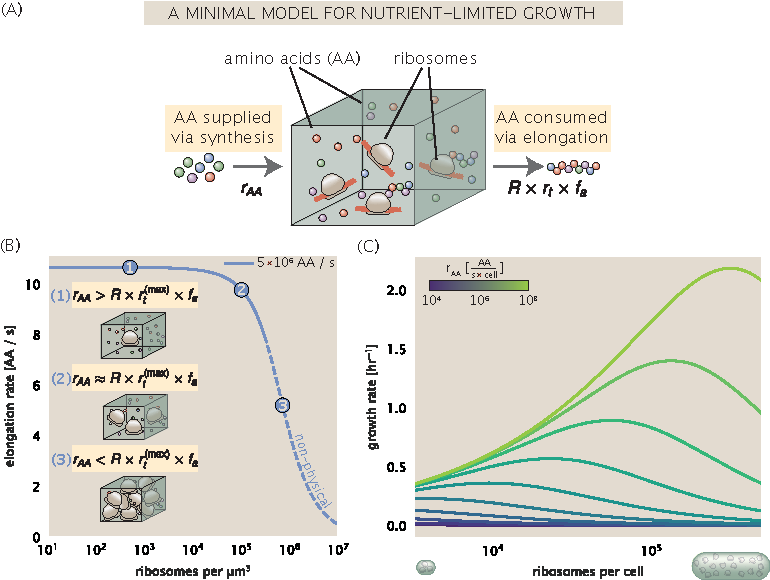
\includegraphics{main_figs/elongation_model.pdf}
        \caption{\textbf{A minimal model of growth rate control under
        nutrient limitation.} (A) We consider a unit volume of cellular material
        composed of amino acids (colored spheres) provided at a supply rate
        $r_{AA}$. These amino acids are polymerized by a pool of ribosomes
        (brown blobs) at a rate $r_t \times R \times f_a$, where $r_t$ is the
        elongation rate, $R$ is the ribosome copy number in the unit volume, and
        $f_a$ is the fraction of those ribosomes actively translating. (B) The
        observed elongation rate is plotted as a function of ribosomes in a unit
        volume \textmu m$^3$. The three points correspond to three regimes of
        ribosome copy numbers and are shown schematically on the left-hand side.
        The region of the curve shown as dashed lines represents a non-physical
        copy number, but is shown for illustrative purposes. This curve was
        generated using the parameters $r_{AA} = 5 \times 10^6$ AA / s, $K_D =
        5$ mM, and $r_t^\text{(max)} = 17.1$ AA / s. (C) The cellular growth
        rate is plotted as a function of total cellular ribosome copy number for
        different cellular amino acid supply rates, with blue and green curves
        corresponding to low and high supply rates, repsectively. As the
        ribosome copy number is increased, so too is the cell volume and total
        protein abundance. We direct the reader to the Suppemental Information
        for discussion  on the inference of the realtionship between cell
        volume, number of peptide bonds, and ribosome copy number.}
        \label{fig:elongation_rate_model}
    }
\end{figure}

\subsubsection{Optimal Growth Rate, Ribosomal Content, and Cell Size Depend on Nutrient
Availability and Metabolic Capacity.}

To relate elongation rate to growth rate, we constrain the set of parameters
based on our available proteomic measurements; namely, we restrict the values of
$R$, $N_{pep}$, and $V$ to those associated with the amalgamated proteomic data
(described in Appendix \nameref{estimate_protein_per_cell}). We then consider
how changes in the nutrient conditions, through the parameter $r_{AA}$,
influence the maximum growth rate as determined by \EQ{lambda_limit}.
\FIG{elongation_rate_model}(C) shows how the observed growth rate depends on the
rate of amino acid supply $r_{AA}$ as a function of the cellular ribosome copy
number. A feature immediately apparent is the presence of a maximal growth rate
whose dependence on $R$ (and consequently, the cell size) increases with
increasing $r_{AA}$. Importantly, however, there is an optimum set of $R$,
$N_{pep}$, and $V$ that are strictly dependent on the value of $r_{AA}$.
Increasing the ribosomal concentration beyond the cell's metabolic capacity has
the adverse consequence of depleting the supply of amino acids and a concomitant
decrease in the elongation rate $r_t$ [\FIG{elongation_rate_model}(B)].

Also of note is the growth rate profiles shown for low amino acid supply rates
[purple and blue lines in \FIG{elongation_rate_model}(C)], representing growth
in nutrient-poor media. In these conditions, there no longer exists a peak in
growth, at least in the range of physiologically-relevant  ribosome copy
numbers. Instead, cells limit their pool of actively translating ribosomes  by
decreasing $f_a$ \citep{dai2016}, which would help maintain the pool of
available amino acids $[AA]_\text{eff}$ and increase the achievable elongation
rate. This observation is in agreement with the central premise of the cellular
resource allocation principle proposed by \cite{scott2010,
klumpp2009,klumpp2014} and \cite{hui2015}.

\section{Discussion}
Continued experimental and technological improvements have led to a treasure
trove of quantitative biological data \citep{hui2015, schmidt2016, si2017,
gallagher2020, peebo2015, valgepea2013}, and an ever advancing molecular view
and mechanistic understanding of the constituents that support bacterial
growth \citep{taheriaraghi2015, morgenstein2015, si2019, karr2012,
kostinski2020, macklin2020}. In this work we have compiled what we believe to be the
state-of-the-art knowledge on proteomic copy number across a broad range of
growth conditions in \textit{E. coli}. We have made this data accessible
through a \href{https://github.com/RPGroup-PBoC/growth_limits}{GitHub
repository}, and an \href{https://rpgroup.caltech.edu/growth_limits//data_explorer}{interactive
figure} that allows exploration of specific
protein and protein complex copy numbers. Through a series of
order-of-magnitude estimates that traverse key steps in the bacterial cell
cycle, this proteomic data has been a resource to guide our understanding of
two key questions: what biological processes limit the absolute speed limit
of bacterial growth, and how do cells alter their molecular constituents as a
function of changes in growth rate or nutrient availability? While not
exhaustive, our series of estimates provide insight on the scales of
macromolecular complex abundance across four classes of cellular processes --
the transport of nutrients, the production of energy, the synthesis of the
membrane and cell wall, and the numerous steps of the central dogma.

In general, the copy numbers of the complexes involved in these processes were
in reasonable agreement with our order-of-magnitude estimates. Since many of these
estimates represent soft lower-bound quantities, this suggests that cells do not
express proteins grossly in excess of what is needed for a particular growth
rate. Several exceptions, however, also highlight the dichotomy between a
proteome that appears to "optimize" expression according to growth rate and one
that must be able to quickly adapt to environments of different nutritional
quality. Take, for example, the expression of carbon transporters. Shown in
\FIG{carbon_tport}(B), we find that cells always express a similar number of
glucose transporters irrespective of growth condition. At the same time, it is
interesting to note that many of the alternative carbon transporters are still
expressed in low but non-zero numbers ($\approx$ 10-100 copies per cell) across
growth conditions. This may relate to the regulatory configuration for many of
these operons, which require the presence of a metabolite signal in order for
alternative carbon utilization operons to be induced \citep{monod1949,
laxhuber2020}. Furthermore, upon induction, these transporters are expressed and
present in abundances in close agreement with a simple estimate.

Of the processes illustrated in \FIG{categories}, we arrive at a
ribosome-centric view of cellular growth rate control. This is in some sense
unsurprising given the long-held observation that \textit{E. coli} and many
other organisms vary their ribosomal abundance as a function of growth
conditions and growth rate \citep{scott2010, metzlraz2017}. However, through our
dialogue with the proteomic data, two additional key points emerge. The first
relates to our question of what process sets the absolute speed limit of
bacterial growth. While a cell can parallelize many of its processes simply by
increasing the abundance of specific proteins or firing multiple rounds of DNA
replication, this is not so for synthesis of ribosomes
[\FIG{ribosome_limit}(A)]. The translation time for each ribosome [$\approx$ 7
min, \cite{dill2011}] places an inherent limit on the growth rate that can only
be surpassed if the cell were to increase their polypeptide elongation rate, or
if they could reduce the total protein and rRNA mass of the ribosome. The second
point relates to the long-observed correlations between growth rate and cell
size \citep{schaechter1958, si2017}, and between growth rate and ribosomal mass
fraction. While both trends have sparked tremendous curiosity and driven
substantial amounts of research in their own regards, these relationships are
themselves intertwined. In particular, it is the need for cells to increase
their absolute number of ribosomes under conditions of rapid growth that require
cells to also grow in size. Further experiments are needed to test the validity
of this hypothesis. In particular, we believe that the change in growth rate in
response to translation-inhibitory drugs (such as chloramphenicol) could be
quantitatively predicted, given one had precision measurement of the relevant
parameters, including the fraction of actively translating ribosomes $f_a$ and
changes in the metabolic capacity of the cell (i.e. the rate that amino acids can be made
available) for a particular growth condition.

While the generation of new ribosomes plays a dominant role in growth rate
control, there exist other physical limits to the function of cellular
processes. One of the key motivations for considering energy production was the
physical constraints on total volume and surface area as cells vary their size
\citep{harris2018, ojkic2019}. As \textit{E. coli} get larger at faster growth
rates, an additional constraint begins to arise in energy production and
nutrient uptake due to the relative decrease in total surface area, where ATP is
predominantly produced \citep{szenk2017}. Specifically, the cell interior
requires an amount of energy that scales cubically with cell size, but the
available surface area only grows quadratically [\FIG{energy_scaling}(A)]. While
this threshold does not appear to be met for \textit{E. coli} cells growing at 2
hr$^{-1}$ or less, it highlights an additional constraint on growth given the
apparent need to increase cell size in order to grow faster. This limit is
relevant even to eukaryotic organisms, whose mitochondria exhibit convoluted
membrane structures that nevertheless remain bacteria-sized organelles
\citep{guo2018}. In the context of bacterial growth and energy production more
generally, we have mainly limited our analysis to the aerobic growth conditions
associated with the proteomic data and further consideration will be needed for
anaerobic growth.1

This work is by no means meant to be a complete dissection of bacterial
growth rate control, and there are many aspects of the bacterial proteome and
growth that we neglected to consider. For example, other recent work
\citep{liebermeister2014, hui2015, schmidt2016} has explored how the proteome is
structured and how that structure depends on growth rate. In the work of
\cite{hui2015}, the authors coarse-grained the proteome into six discrete
categories being related to either translation, catabolism, anabolism, and
others related to signaling and core metabolism. The relative mass fraction of
the proteome occupied by each sector could be modulated by external application
of drugs or simply by changing the nutritional content of the medium. While we
have explored how the quantities of individual complexes are related to cell
growth, we acknowledge that higher-order interactions between groups of
complexes or metabolic networks at a systems-level may reveal additional
insights into how these growth-rate dependences  are mechanistically achieved.
Furthermore, while we anticipate the conclusions summarized here are applicable
to a wide collection of bacteria with similar lifestyles as \textit{E. coli},
other bacteria and archaea may have evolved other strategies that were not
considered. Further experiments with the level of rigor now possible in
\textit{E. coli} will need to be performed in a variety of microbial organisms
to learn more about how regulation of proteomic composition and  growth rate
control has evolved over the past 3.5 billion years.

%
%
%
%
% our estimates are
% appear to be in excess of what would be minimally required to support cell
% growth at the observed rates.
%
%
%  to elucidate a
% fundamental question in bacterial physiology -- what sets the speed limit at
% which cells can divide?


%
% Recent years have seen an explosion in our understanding of the cellular
% macromolecular composition at unprecedented resolution. This quantitative,
% molecular view of cell biology has transformed our understanding of how and when
% genes are expressed, to what degree they are expressed, and precisely how they
% are post-translationally modified (a topic we have not considered in this work,
% but appreciate nonetheless). Despite these impressive studies, an understanding
% of how the abundance and regulation is related to growth rate has been largely
% treated with phenomenological models, often containing obscure dimensionless
% parameters or polynomial fits to data. While these phenomenological treatments
% have revealed fascinating features of the resource allocation within the
% proteome, elucidating the molecular details of \textit{how} these resource
% allocation strategies operate has remained enigmatic.
%
% In this work, we present a series of order-of-magnitude estimates to elucidate a
% fundamental question in bacterial physiology -- what sets the speed limit at
% which cells can divide?
%
%
% Countless careers have been built examining the minutiae of each of
% the processes listed in \FIG{categories}, resulting in a treasure
% trove of literature representing decades of careful experimentation, modeling,
% and interpretation of results. Despite the undeniable complexity of each
% individual process, our work illustrates that in order to understand what sets
% the scale of the observed protein copy numbers and their corresponding
% dependence on growth rate, a coarse-grained view of the system is often
% appropriate.
%
%
% [GC: Other topics to discuss include the utility of scrounging the data from the
% literature to assemble, to our knowledge, the most complete view of the
% condition-dependent proteome of \textit{E. coli}.]
%
%
% [Fill in.]

% Parallelized DNA replication represents a solution that allows  \textit{E. coli}
% to synthesize enough rRNA as it grows faster. That the cell appears to
% be synthesizing rRNA near its maximal rate at growth rates above about 0.5 h$^{-1}$
% may also have consequences on robust scaling  between
% cell size and $\langle$\# ori$\rangle$. As one example, when cells are exposed
% to sublethal doses of ribosome-inhibiting drugs like chloramphenicol, there is a
% notable increase in the cell's ribosomal fraction (grey points,
% \FIG{translation_ecoli_partA}(D)), but otherwise the cell is able to maintain
% its cell size according to $\langle$\# ori$\rangle$ \citep{si2017}. While the
% presence of chloramphenicol will inhibit protein synthesis, it will also allow
% for relatively higher rRNA synthesis due to the longer doubling time. If the
% cell can scale it ribosomal protein abundance through feedback from rRNA
% synthesis, than we would expect the relative abundance of ribosomes to increase
% according to the increase in rRNA synthesis. This type of feedback was
% considered long ago \citep{nomura1984} and we consider this possibility further
% in Supplemental Appendix XX.


% While it is difficult to distinguish between causality and correlation, the data
% also helps us resolve why cell size, should exhibit an exponential increase with growth
% rate once cells begin to parallelize DNA replication. Specifically,
%
% is consistent with the need for cells to increase their effective rRNA gene
% dosage in order to grow according to the constraint set by Equation 2. Importantly, it
% may also shed some light on the notable increase in ribosomal content
% that is observed when sublethal doses of antibiotics \citep{scott2010, dai2016}.
% Specifically, if rRNA synthesis is rate limiting, and nutrient conditions
% largely dictate the extent of overlapping DNA replication cycles, than addition
% of antibiotic will lengthen the doubling time and allow increased rRNA
% synthesis relative to the rate of cell division. In Supplemental Section XX, we
% consider this further using additional data from \cite{si2017}.


% A number of recent papers further highlight the possibility that regulation
% (p)ppGpp may be the critical component of the apparent scaling laws in
% \textit{E. coli}. In the context of ribosomal activity, increased levels of
% (p)ppGpp are associated with lower ribsomal content, and at slow growth
% are associated with reduced activity by ribosomes and RNA polymerse \citep{dai2016,
% dai2018} [citations for RNAP]. Titration of the cellular (p)ppGpp concetrations (up or down) can
% invoke similar proteomic changes reminiscent of those observed under nutrient
% limitation \citep{zhu2019}. In light of the limiting dependence of ribosome copy
% number on chromosomal gene dosage, it was recently shown that growth in a
% (p)ppGpp null strain abolishes both the scaling in cell size  and the
% $\langle$\# ori$\rangle$ / $\langle$\# ter$\rangle$ ratio. Instead, cells
% exhibited a high $\langle$\# ori$\rangle$ / $\langle$\# ter$\rangle$ closer to 4
% and cell size more consistent with a fast growth state where (p)ppGpp levels are
% low \citep{fernandezcoll2020}. From these results, perhaps the perspective to
% take is that the scaling laws  reflect an attempt for the cell to mitigate its
% biological activity according  to available nutrients.

\section{Methods}

\subsection{Data Analysis and Availability}
All proteomic measurements come from the experimental work of \cite{schmidt2016,
peebo2015, valgepea2013} (mass spectrometry) and \cite{li2014} (ribosomal
profiling). Data curation and analysis was done programmatically in Python, and
compiled data and analysis files are accessible through a
\href{https://github.com/rpgroup-pboc/growth_limits}[GitHub repository]
(DOI:XXX) associated with this paper as well as on the associated
\href{https://rpgroup.caltech.edu/growth_limits}{paper website}. An interactive
figure that allows exploration of specific protein and protein complex copy
numbers is available at [link].


% Here we can note that data was collected, curated, and is available on Github, and whatever minimal details we might want to include.

\section{Acknowledgements}
We thank Matthias Heinemann, Alexander Schmidt, and Gene-Wei Li for additional
input regarding their data. We also thank members of the Phillips, Theriot,
Kondev, Garcia labs, as well as Ron Milo and Terry Hwa for useful discussions.
We thank Suzannah M. Beeler, Avi Flamholz, Soichi Hirokawa, and Manuel
Razo-Mejia for reading and providing comments on drafts of this manuscript. R.P.
is supported by La Fondation Pierre-Gilles de Gennes, the Rosen Center at
Caltech, and the NIH 1R35 GM118043 (MIRA). J.A.T. is supported by the Howard
Hughes Medical Institute, and NIH Grant R37-AI036929. N.M.B is a HHMI Fellow of
The Jane Coffin Childs Memorial Fund. H.G.G. is supported by the Burroughs
Wellcome Fund Career Award at the Scientific Interface, the Sloan Research
Foundation, the Human Frontiers Science Program, the Searle Scholars Program,
the Shurl \& Kay Curci Foundation, the Hellman Foundation, the NIH Director’s
New Innovator Award (DP2 OD024541-01), and an NSF CAREER Award (1652236). D.S.F.
is supported by an NSF award (PHY-1607606).

\section{Competing Interests}
The authors declare no competing interests.




%  \newpage
%%%%%%%%%%%%%%%%%%%%%%%%%%%%%%%%%%%%%%%%%%%%%%%%%%%%%%%%%%%%
%%% Bib START
%%%%%%%%%%%%%%%%%%%%%%%%%%%%%%%%%%%%%%%%%%%%%%%%%%%%%%%%%%%%
\bibliography{./library.bib}
\end{document}
